% =====================================================================
% SEMI-DEPRECATED. main-lean.tex is CANONICAL for all ported content.
% This file is retained for material not yet ported (full proofs, extended
% simulations/application). Its Path 3 framing is STALE: §4.1 ("General
% framework") still presents all three paths as theta_gt = f(g,I_t;theta)
% and Path 3 as inverting the marginals — superseded. The canonical Path 3
% (direct CATE estimation + covariate transport, doubly-robust EIF) lives
% in main-lean.tex §4 (Path 3: Covariate Transport) and §5. Do not treat
% this file's Path 3 / general-framework as current. See
% quality_reports/2026-06-30_phase1-path3-theory-note.md.
% =====================================================================
\documentclass{article}
\usepackage{graphicx} % Required for inserting images
\usepackage{amsmath, amsfonts, amssymb, amsthm}
\usepackage{color, xcolor}
\usepackage{setspace}
\usepackage{natbib}
\usepackage{booktabs}
\title{What we estimate when we estimate dynamic causal effects in panel data}
\date{\today}
\input{common-defs}
\input{typography-preamble}

\newtheorem{assumption}{Assumption}
\newtheorem*{proposition*}{Proposition}
\newtheorem*{lemma*}{Lemma}

\setlength{\topmargin}{-.25in}
\setlength{\oddsidemargin}{-0.4in}
\setlength{\textwidth}{7.2in}
\setlength{\textheight}{9.0in}
\setlength{\unitlength}{1em}
\parindent 16pt

\renewcommand{\P}{\mathbb{P}}

\doublespacing

\begin{document}

\maketitle

\begin{abstract}
Policy-relevant decisions depend on causal effects in the current or next period (e.g., FATT, FATU), but standard panel-data methods target backward-looking estimands such as the average treatment effect on the treated (ATT) or group-time ATTs over the observed window. We formalize this gap using future causal effects and present three identification strategies. Taking dynamic effects \emph{less} seriously, the FATT is identified under time homogeneity by the ATT or by a convex combination of within-group ATTs (Path~1). Taking them \emph{more} seriously, the FATT is identified either by specifying how group-time effects evolve and extrapolating (Path~2), or by modeling structural heterogeneity via covariates and integrating over the future covariate distribution (Path~3). Path~3 enables identification under regime change when reduced-form temporal patterns break but structural covariates remain predictive. For Path~2, we provide the first systematic framework for model selection in causal extrapolation, using time-series cross-validation to test extrapolation performance rather than in-sample fit. We give efficient influence functions for the FATT under all three paths so that standard errors and confidence intervals propagate correctly from first-stage estimators.
\end{abstract}

\section{Introduction}

There is a fundamental and unacknowledged tension at the heart of policy analysis and causal inference with panel data more broadly \citep{egamiElementsExternalValidity2023,heckmanPolicyRelevantTreatmentEffects2001}. This tension arises because of the possibility of dynamic causal effects (effects that change over time), which, as we'll argue below, preclude an important type of external validity: if policy effects are truly unrestrictedly dynamic, then it is impossible to use historical data to inform \textit{any} current decisions, which decisions are presumably the reason we care about estimating any causal effects in the first place.

Most causal inference rests on an implicit assumption of time homogeneity. We might call this assumption the Fundamental Promise of Causal Inference: causal effects estimated (by necessity) on data collected in the past can be used to inform decision-making in the present \citep{egamiElementsExternalValidity2023,khosrowiExtrapolationCausalEffects2019,cartwrightHuntingCausesUsing2007}. If two identical clinical trials -- same target population and inclusion criteria, same treatment, same outcome -- were expected to not only give different results but in fact target different causal effects simply because of the passage of time, that would be a major crisis for causal inference. A durable understanding of causal effects would be elusive.

Public policies are widely understood to violate this assumption and are assumed to have effects that inherently change over time \citep{lucasjrEconometricPolicyEvaluation1976,ericssonExogeneityCointegrationEconomic1998,estrellaAreDeepParameters1999}. Policies are introduced into dynamic contexts, may be administered or enforced differently over time, and may themselves cause changes in public behavior and attitude. Technological advancement, public opinion, economic conditions, and new research may all modify the causal effects policies.

This basic assumption of dynamic effects has driven a great deal of recent advances in methods for causal inference with panel data \citep{sunEstimatingDynamicTreatment2021,wangAdvancesDifferenceindifferencesMethods2024a}. Recent surveys clarify how heterogeneity and dynamics enter identification and estimation in this setting \citep{arkhangelskyCausalModelsLongitudinal2024,dechaisemartinTwowayFixedEffects2023}. It is now standard to assume that causal effects vary both with time of treatment and time since implementation. These effects (often called ``group-time" effects) may be of interest in themselves but more typically are aggregated into coarser effects like an ``overall" average treatment effect on the treated (ATT). Assuming such dynamic effects solves a problem with classical methods like two-way fixed effects: they may incur bias in the presence of time-heterogeneous effects because they implicitly include comparisons between units treated at different times in their estimate of the ATT \citep{sunEstimatingDynamicTreatment2021}.

While methods assuming dynamic effects have been developed for good reasons, they strike at the heart of the Fundamental Promise of Causal Inference. In the presence of dynamic effects, it is not clear how one can connect causal effects estimated on historical data to any decision one would make now or in the future \citep{egamiElementsExternalValidity2023,devauxQuantifyingRobustnessExternal2022,khosrowiExtrapolationCausalEffects2019}. The question of when and how historical evidence can inform current or future decisions is central to the literature on generalizing and transporting causal effects \citep{coleGeneralizingEvidenceRandomized2010,tiptonImprovingGeneralizationsExperiments2013,manskiPublicPolicyUncertain2013}. If one estimates the effect of a public policy to be beneficial (e.g., improves life expectancy) among states that implemented it in historical data, does that mean that it would be wise to maintain that policy in places that have already implemented and/or to implement it in places it has not been implemented? If effects are unrestrictedly dynamic, it's impossible to say. 

We seek to resolve this tension between dynamic effects and the Fundamental Promise by encouraging researchers to either take the possibility of dynamic effects \textit{less} seriously or \textit{more} seriously---and, when taking them more seriously, to choose what they believe is invariant. Taking it less seriously (Path~1) involves assuming some level of time homogeneity in causal effects. This would allow causal effects that would inform current and future decisions to be identified in historical data. We argue that an informal version of this is currently standard practice, where average treatment effects estimated on historical data are treated as if they are stable enough over time to inform current debates \citep{gablerDealingHeterogeneityTreatment2009,cintronHeterogeneousTreatmentEffects2022}. The notion of policy-relevant treatment effects formalizes which estimands answer counterfactual policy questions \citep{heckmanPolicyRelevantTreatmentEffects2001,sasakiEstimationInferencePolicy2023}. On the other hand, taking dynamic effects more seriously would require formally modeling how effects change over time. Under Path~2, researchers specify temporal dynamics (e.g., trends in event time) and extrapolate \citep{khosrowiExtrapolationCausalEffects2019,maebaExtrapolationTreatmentEffect2024}. Under Path~3, researchers model structural heterogeneity via covariates and integrate over the future covariate distribution. Path~3 is robust to regime change if treatment effects are driven by observable covariates that capture ``deep parameters'' \citep{lucasjrEconometricPolicyEvaluation1976}---even when reduced-form temporal patterns break, structural covariates may remain predictive. This approach connects to structural methods that enable extrapolation across regimes \citep{heckmanStructuralEquationsTreatment2005,pearlExternalValidityCalculus2022}.

We introduce new causal estimands that formalize the notion that causal inference is inherently future-oriented, which we call ``future causal effects." We locate the estimands outside the time range of the current study and present three identification paths that differ in what they assume is invariant: Path~1 assumes temporal stability of effects; Path~2 assumes a functional form for temporal dynamics; Path~3 assumes structural covariates remain predictive under regime change. Across fields, three broad strategies emerge for making causal claims about the future: structural or parameter invariance (e.g., policy-invariant deep parameters); statistical transport or reweighting of effects across populations; and explicit modeling of heterogeneity or dynamics. Our three paths map cleanly onto these traditions, with Path~3 most directly invoking the Lucas critique's emphasis on structural parameters.

\subsection{Related work}

Recent advances in causal inference for panel data and difference-in-differences provide the backbone for our setting. Surveys by \citet{arkhangelskyCausalModelsLongitudinal2024} and \citet{dechaisemartinTwowayFixedEffects2023} clarify how heterogeneity and dynamics enter identification and estimation; the group-time and staggered-adoption literature \citep{callawayDifferenceindifferencesMultipleTime2021,sunEstimatingDynamicTreatment2021,rothEfficientEstimationStaggered2023,bakerDifferenceinDifferencesDesignsPractitioners2025} addresses inference for backward-looking effects when treatment timing varies. Work on testing parallel trends and time homogeneity---including the limitations of conventional pre-trend tests \citep{freyaldenhovenPreeventTrendsPanel2019}, the pitfalls of conditioning on passing such tests \citep{rothPretestCautionEventstudy2022}, inference under bounded trend violations \citep{rambachanMoreCredibleApproach2023}, and equivalence tests for pre-trends \citep{detteTestingEquivalencePreTrends2024}---connects directly to the testable implications of our time-homogeneity assumptions. These lines of work focus on identification and inference for effects in the observed window; we instead target estimands that are relevant for current or future policy decisions.

The disconnect between typical estimands (ATT, group-time effects) and policy-relevant or future causal questions has been formalized in several ways. \citet{heckmanPolicyRelevantTreatmentEffects2001} define policy-relevant treatment effects for counterfactual policy changes; \citet{sasakiEstimationInferencePolicy2023} provide estimation and inference for such parameters. \citet{forastiereForecastingCausalEffects2025} formalize forecasting the causal effect of \emph{re-implementing} an intervention at a future time; we focus on the effect of the policy in the current or next period ($p+1$)---continuing or repealing for current adopters, adopting or not for non-adopters---and potentially beyond. \citet{gischeForecastingCausalEffects2021} distinguish forecasting the causal effect of an intervention from predicting future outcomes; we similarly distinguish backward-looking estimands (e.g., the ATT in the observed window) from forward-looking, policy-relevant estimands such as the FATT and FATU at time $p+1$. \citet{debCounterfactualForecastingPanel2026} forecast unit-level counterfactual outcomes by imposing autoregressive dynamics on latent factors in a matrix completion framework; our approach instead directly targets population-level causal effects under weaker structural assumptions and accommodates regime change. \citet{shenControlTreatmentCausal2026} extends synthetic control and synthetic interventions to forecast a single control unit's treated-state trajectory one or a few periods beyond the observed panel, imposing a shared invariant unit factor and low-rank Hankel structure on latent temporal factors and establishing pointwise asymptotic normality via a debiased principal-component-regression estimator; the estimand there is a unit-level potential outcome for an already-known target unit rather than a population-level group-time ATT, and neither the identification strategy nor the estimator engages with the group-time ATT or efficient-influence-function machinery underlying our three paths.

External validity and transportability are central to our concern that backward-looking estimands may not inform current decisions. \citet{egamiElementsExternalValidity2023} provide a framework for design and analysis; \citet{pearlExternalValidityCalculus2022} and \citet{bareinboimTransportabilityCausalEffects2012} give graphical and identification results for transporting causal effects. The literature on generalizing from randomized trials to target populations \citep{coleGeneralizingEvidenceRandomized2010,tiptonImprovingGeneralizationsExperiments2013} and on robustness to external validity bias \citep{devauxQuantifyingRobustnessExternal2022} is closely related. \citet{khosrowiExtrapolationCausalEffects2019} and \citet{khosrowiExtrapolatingExperimentsConfidently2023} examine the assumptions and uncertainties underlying extrapolation; \citet{manskiPublicPolicyUncertain2013} advocates bounded identification when extrapolation is weak. \citet{shpitserCounterfactualGraphicalModels2013} extend transportability to longitudinal settings.

The Lucas Critique and the question of policy invariance underlie our discussion of when effects can be taken as stable over time. \citet{lucasjrEconometricPolicyEvaluation1976} argues that policy evaluation requires parameters that are invariant to the policy regime; \citet{ericssonExogeneityCointegrationEconomic1998} and \citet{estrellaAreDeepParameters1999} formalize and test such invariance. Structural and parametric approaches to extrapolation---including \citet{heckmanStructuralEquationsTreatment2005} on policy-invariant parameters, \citet{pearlExternalValidityCalculus2022} on transportability, and \citet{brodersenInferringCausalImpact2015} on Bayesian structural time series---show how functional assumptions enable extrapolation across regimes or time periods.

Philosophical work on causal invariance and extrapolation \citep{cartwrightHuntingCausesUsing2007} and empirical evidence on heterogeneous treatment effects in policy and program evaluation \citep{gablerDealingHeterogeneityTreatment2009,cintronHeterogeneousTreatmentEffects2022} further motivate the need to be explicit about which effects are policy-relevant and under what assumptions they can be identified from historical data.

Our future-looking estimands sit at the intersection of three strategies for making causal claims about the future: structural or parameter invariance, statistical transport or reweighting, and explicit modeling of heterogeneity or dynamics.

% \begin{itemize}
%     \item Classical causal inference imagines a stable treatment.
%     \item The effect of a drug may vary with patient characteristics, but we implicitly assume when we run clinical trials that the effect of the drug will not typically change just because of the passage of time. It doesn't matter when the clinical trial is run, it will still inform the effectiveness of the drug today.
%     \item Policies are different -- their effects may change over time for lots of reasons... implementation, enforcement, public behavior, etc.
%     \item Recent advances in causal inference for panel data (the typical approach for studying policies) have been directly targeted at addressing issues of time heterogeneity.
%     \item However, there is a contradiction at the heart of these analyses: if the effects of the policy can change unrestrictedly over time, the classical paradigm completely breaks down. Causal effects based on historical data cannot be immediately used to infer the effect of the policy today, the only time we really care about.
%     \item We propose two ways of resolving this contradiction: either take time heterogeneity more or less seriously.
%     \item Less seriously: assume some form of time homogeneity that identifies the effect of the policy today with something that can be estimated with historical data. This is the spirit in which most estimated policy effects appear to be interpreted today: if the causal effect on historical data is found to be positive, it is assumed that the effect of the law today will be broadly positive.
%     \item More seriously: model how the policy changes over time and extrapolate policy effects to today.
%     \item Something about how we define new causal effects and why that's needed for this paper.
% \end{itemize}

\section{Setting and context}\label{context}

Suppose we measure an indicator of a policy $A_{it}$, a possibly affected outcome $Y_{it}$, and pre-treatment covariates $\bX_{it}$---which may be time-invariant or time-varying---for $i = 1, ..., n$ units (often the units are geographic entities, like states, counties, etc.) and $t = 1, ..., p$ timepoints. We write $\bX_i$ when covariates are time-invariant or when the period is clear from context; the distinction matters for Path~3 (Section~\ref{sec:path3}), where a shifting covariate distribution is the engine of extrapolation. For ease of exposition, we take $A_{it}$ to be a policy, but all that follows applies equally to other types of interventions. Define the counterfactual value that $Y_{it}$ would take if the policy were set, possibly contrary to fact, to $A_{it} = a$ as $Y_{it}(a)$. We assume no interference: each unit's potential outcomes depend only on that unit's treatment, so $Y_{it}(a)$ is well-defined. We further assume throughout that the covariates $\bX_{it}$ used for adjustment are \emph{unaffected by the policy}---pre-treatment or otherwise externally determined, so that $\bX_{it}$ does not lie on a causal path from treatment to outcome. With time-invariant baseline covariates this holds automatically; it is the standard condition underlying covariate adjustment in any first-stage design and is invoked again by Path~3 (Section~\ref{sec:path3}), which integrates over a \emph{future} covariate distribution. When covariates are time-varying \emph{and} affected by treatment, valid adjustment requires g-methods \citep{robinsNewApproachCausal1986}; we assume exogeneity and leave that case to future work. Let $\cO = \{\bX_i, \bY_{i}(0), \bY_{i}(1), \bA_{i}\}_{i = 1, ..., n} \sim \P$ where $\bY_i(a) = \{\bY_{it}(a)\}_{t = 1, ..., p}$ and $\bA_i = (A_{it})_{t = 1,.., p}$. We extend the setting to future time periods when defining future estimands below. The distribution of data at time $t$ is $\P_t$. For integer $k \geq 1$, we write $\P_{p+k}$ for the distribution of $(\bX_i, Y_{i,p+k}(0), Y_{i,p+k}(1), A_{i,p+k})$ in the same superpopulation $k$ periods ahead (i.e., the marginal at $t = p+k$ of the joint distribution governing the process through $p+k$); $\P_{p+1}$ is the case $k=1$. 

It is typical (though not necessary) in such studies to take the target of estimation to be the average treatment effect on the treated (ATT). The ATT may be defined as
\begin{align*}
    \theta = \E_\P\{Y_{it}(1) - Y_{it}(0) | A_{it} = 1\}.
\end{align*}
One virtue of the ATT is that $Y_{it}(1)$ is always observed under the conditioning event $A_{it} = 1$, so identification of the ATT is facilitated by only requiring causal inference machinery to estimate $\E_\P\{Y_{it}(0) | A_{it} = 1\}$.

In the presence of heterogeneity -- especially heterogeneity in how policy effects change over time -- there have been proposals to instead decompose the ATT into separate sub-ATTs, with an example being referred to as group-time ATTs \citep{sunEstimatingDynamicTreatment2021}.
\begin{align*}
    \theta_{gt} = \E_{\P_t}\{Y_{it}(1) - Y_{it}(0) | A_{it} = 1, G_{i} = g\}
\end{align*}
where $G_i = \min\{t : A_{it} = 1\}$ (with $G_i = \infty$ if the policy is never adopted), the time when the policy first occurred, and $\P_t$ is the distribution of the data at time $t$: $\cO_t = \{\bX_i, Y_{it}(0), Y_{it}(1), A_{it}\}_{i = 1, ..., n} \sim \P_t$. This is important to solve some infelicities with trying to estimate $\theta$ directly with a single linear model \citep{sunEstimatingDynamicTreatment2021} and to draw attention to the fact that causal effects may both vary across calendar time and have different effects as implementation continues -- i.e., effects may differ in the first year of implementation from the fifth year, say. These sub-ATTs are typically then aggregated up into an overall effect estimate across groups/times.

\begin{assumption}[Absorbing adoption]\label{absorbing-adoption}
For every unit $i$ and every $t \in \{1,\ldots,p\}$, $A_{it} = 1$ implies $A_{is} = 1$ for all $s \in \{t+1,\ldots,p+1\}$.
\end{assumption}

Assumption~\ref{absorbing-adoption} states that adoption is permanent over the window under study: a policy in force at $t$ remains in force through $p+1$, so $G_i = \min\{t : A_{it}=1\}$ records the single date at which unit $i$ transitions, and $A_{it} = \mathbf{1}\{G_i \leq t\}$. What it rules out is repeal and reinstatement within $\{1,\ldots,p+1\}$; it says nothing about which units adopt or when. Assumption~\ref{absorbing-adoption} is maintained throughout and is the only assumption behind Lemmas~\ref{lem:persistence} and~\ref{lem:aggregation} below.

\subsection{Identification of the backward-looking ATT}
The results in Section~\ref{sec:general-framework} (covering all three identification paths) assume that the researcher has secured identification of the ATT $\theta$ and, where relevant, the group-time ATTs $\theta_{gt}$, under some design. For example, under parallel trends in difference-in-differences, $\theta_{gt}$ is identified from the observed data \citep{callawayDifferenceindifferencesMultipleTime2021,sunEstimatingDynamicTreatment2021}; under unconfoundedness or other designs, different identification formulas apply. We do not restrict the first-stage identification strategy: it may be difference-in-differences, synthetic control, or another approach. The contribution of this paper is to show when and how these backward-looking estimands coincide with or can be used to identify the policy-relevant FATT (and related future estimands), given time homogeneity assumptions (Path~1, Section~\ref{sec:path1}), a parametric model for dynamics (Path~2, Section~\ref{sec:path2}), or structural covariate-driven effects (Path~3, Section~\ref{sec:path3}). Thus the full identification argument has two steps: (a) under the researcher's design, $\theta$ or $\theta_{gt}$ are identified from observables; (b) under the extrapolation assumptions we state below, the FATT is identified from $\theta$ or $\theta_{gt}$.

However, regardless of how they are aggregated, these effects are typically not directly relevant to current policy or decisionmaking \citep{egamiElementsExternalValidity2023,khosrowiExtrapolationCausalEffects2019}. These ATTs necessarily correspond to what has happened \textit{in the past}. While assessing the effects of policies in the past may have some utility -- e.g., for electoral purposes -- for a decisionmaker considering implementing a new policy or repealing a policy that is currently on the books, these backward-looking estimands are not germane without further assumptions. 

% We suggest that an example of a more relevant estimand is the future average treatment effect on the untreated (FATU)
% \begin{align*}
%     \omega_{p+1} = \E_{\P_{p+1}}\{Y_{i,p+1}(1) - Y_{i,p+1}(0) | A_{ip} = 0\}.
% \end{align*}
% The future ATU corresponds to the average value of the outcome if all units that currently (as of the end of the study period) did not have the policy were to implement it in time $p+1$ compared to if they remained without the policy. This estimand is relevant for any policymakers who are considering whether this policy might be right for their unit. Unlike the ATT and sub-ATTs above, none of the counterfactuals are observed, and in fact we lack any direct knowledge of the distribution of $\P_{p+1}$. 

% This disconnect between policy-relevant quantities and typical estimands like the ATT has largely been implicit in the policy analysis and causal inference literatures. We argue that settling for backwards-looking ATTs to inform future policy implementation is like looking for one's keys under the streetlight. Below we define a range of novel potentially forward-looking, policy-relevant estimands, we discuss under what circumstances these novel estimands correspond to commonly-used backwards-looking estimands like the ATT, and we further outline under what assumptions these novel estimands may be identified when they do not correspond to backwards-looking estimands.

\section{Estimands}
We require more policy-relevant estimands that are future-looking and correspond to ``future causal effects." These estimands are designed to address actual policy decisions: should we implement or repeal this policy? We define them for a generic horizon $k \geq 1$ (i.e., $k$ periods ahead); conditioning on treatment status is at the end of the study period $p$ (e.g., effect for current adopters or non-adopters at horizon $k$).

Let 
\begin{align*}
    \tau_{i,p+k} = Y_{i,p+k}(1) - Y_{i,p+k}(0)
\end{align*} 
be the future individual treatment effect (FITE) for unit $i$ at horizon $k$. The FITE is arguably the most relevant quantity for a citizen or policymaker belonging to unit $i$. For example, state lawmakers in California may likely be interested most in the FITE for California. The fact that individual treatment effects are not as a rule identifiable does not change the fact that it may be what is of primary importance. The FITE motivates the population-level estimands below but is not itself a target we identify; likewise none of the future causal effects in this section are identifiable from the observed data without further assumptions.

Given the difficulties with estimating individual treatment effects, we may consider an alternative, the future average treatment effect among similar units (FATS). Given a distance measure $\rho$, we can define:
\begin{align*}
    \tau_{i,p+k}(\eta; \rho) = \E_{\P_{p+k}}\left\{Y_{j,p+k}(1) - Y_{j,p+k}(0) | \rho(\bX_i, \bX_j) \leq \eta \right\}
\end{align*} 
i.e., the average treatment effect at $p+k$ among units $j$ such that $\rho(\bX_i, \bX_j) \leq \eta$; similarity is defined by distance in covariate space. (The backward-looking analog is the ATS: the average effect among units in that same set of units, under $\P_t$.) For example, policymakers in Massachusetts may be interested in the treatment effect among states in New England, or New York policymakers may be interested in the effect among other high-population states. Like the FITE, the FATS serves to motivate the policy questions; we treat it as a localized version of the population estimands below (recovered by restricting the target covariate distribution to a neighborhood of $\bX_i$) rather than as a separate object of study.

When policymakers do not have a unit-specific focus, other treatment effects may be of interest. Consider the future-looking analogs of typical backward-looking estimands at horizon $k$:
\begin{align*}
    \tau_{p+k} &= \E_{\P_{p+k}}\{Y_{i,p+k}(1) - Y_{i,p+k}(0)\} & (FATE)\\
    \theta_{p+k} &= \E_{\P_{p+k}}\{Y_{i,p+k}(1) - Y_{i,p+k}(0) | A_{ip} = 1\} & (FATT)\\
     \omega_{p+k} &= \E_{\P_{p+k}}\{Y_{i,p+k}(1) - Y_{i,p+k}(0) | A_{ip} = 0\} & (FATU)
\end{align*}
The FATE encodes the average outcome at time $p+k$ if all units implemented or continued the policy compared to if all units discontinued or remained without the policy. The FATE is similar to the average treatment effect (ATE), and considers the most extreme counterfactual scenario of all implementing units versus none. The FATT encodes the difference in average outcome for units with the policy implemented at time $p$ (the end of the study period)
if they continued the policy compared to if they discontinued the policy at time $p+k$. The FATT is analogous to the ATT and is targeted at the effect of repealing the policy. The FATU similarly encodes the difference in average outcome among units without the policy at time $p$ if they newly implemented the policy compared to if they remained without at time $p+k$. The FATU is most relevant to policymakers considering whether they should implement the policy. 

These three estimands---FATT, FATU, and FATE---are the policy-relevant family we carry through the paper. They map directly to the three decisions a policymaker faces: whether to \emph{repeal} a policy currently in place (FATT), whether to \emph{adopt} one not yet in place (FATU), and the effect of \emph{universal} adoption (FATE). They also share identification machinery: each is the future conditional effect $\tau(x)$ averaged over a different target covariate distribution (treated units, untreated units, or the whole population), a structure we exploit directly in Path~3 (Section~\ref{sec:path3}) and which the FATE/FATU recover from the FATT via the relationships above. We develop identification primarily for the FATT and indicate throughout how the FATU and FATE follow.

Unlike the ATT and sub-ATTs above, none of the counterfactuals are observed. In fact, unlike for any backward-looking estimand, we lack any direct knowledge of the distribution of $\P_{p+k}$. We therefore require additional machinery to connect the observed data to the policy-relevant distribution $\P_{p+k}$. We outline below two different options: either taking time heterogeneity \textit{less} seriously -- by making time homogeneity assumptions -- or taking it \textit{more} seriously and formally modeling how policy effects change. \textbf{In the remainder of the paper we take $k=1$ (one period ahead);} extension to $k > 1$ is analogous and noted where it differs.

\section{Identification via Extrapolation Functions}

Forward-looking estimands like the FATT at $p+1$ require extrapolation beyond the observed data. The three identification paths we present can be unified under a single conceptual framework: each path specifies an \emph{extrapolation function} $f$ and assumes that some structural relationship is invariant across time. What differs across paths is the choice of $f$---what it depends on and what is assumed stable.

\subsection{General framework}\label{sec:general-framework}

% STALE FRAMING (semi-deprecated): the "all three paths express theta_gt =
% f(g,I_t;theta)" device below is superseded. It does not hold for Path 3,
% which estimates the conditional effect tau(x) directly and never passes
% through the marginal theta_gt. Canonical framing ("what is held invariant")
% is in main-lean.tex §4. Retained here only because downstream proofs/sims
% in this file reference it.

All three paths share a common principle: they express the group-time treatment effects $\theta_{gt}$ as a function of parameters and ``information'' available at time $t$, then extrapolate this relationship to $t = p+1$. Formally, we write
\begin{align*}
\theta_{gt} = f(g, \mathcal{I}_t; \btheta), \quad t = 1, \ldots, p,
\end{align*}
where $f(\cdot)$ is an extrapolation function, $\mathcal{I}_t$ represents available information at time $t$, and $\btheta$ are parameters identified from the observed $\{\theta_{gt}\}_{t \leq p, g \in \cG}$. The FATT is then
\begin{align*}
\theta_{p+1} = \sum_{g \in \cG} \omega_g f(g, \mathcal{I}_{p+1}; \btheta),
\end{align*}
where $\omega_g = \Prob(G_i = g | A_{ip} = 1)$ is the probability of cohort $g$ among units treated by period $p$.

The three paths differ in their specification of $f$ and $\mathcal{I}_t$:

\begin{table}[h]
\centering
\caption{Three identification paths as choices of extrapolation function}
\label{tab:three-paths}
\begin{tabular}{llll}
\toprule
\textbf{Path} & \textbf{Function $f$} & \textbf{Input $\mathcal{I}_t$} & \textbf{What's Invariant} \\
\midrule
1 & $\gamma_g$ (constant in $t$) & Group index only & Group-specific effects \\
2 & $f(g,t; \bgamma)$ & (Group, Time) & Temporal functional form \\
3 & $\int m(x; \bbeta) \, dF_{\bX}^t(x)$ & Covariate dist.\ at $t$ & Conditional effect $m(x; \bbeta)$ \\
\bottomrule
\end{tabular}
\end{table}

\begin{itemize}
    \item \textbf{Path 1 (time homogeneity):} $f$ is constant over time within each group; $\mathcal{I}_t$ contains only the group index $g$. This assumes group-specific treatment effects do not change over time.

    \item \textbf{Path 2 (parametric extrapolation):} $f$ is a parametric function of group and time (or event time $k = t - g$); $\mathcal{I}_t$ encodes temporal dynamics. This assumes effects follow a smooth functional form that continues into the future.

    \item \textbf{Path 3 (covariate integration):} $f$ depends on the covariate distribution $F_{\bX}^t$ at time $t$; $\mathcal{I}_t$ is the population composition. This assumes the conditional effect $\tau(x) = m(x; \bbeta)$ is invariant, even if the covariate distribution shifts.
\end{itemize}

\paragraph{General identification principle.} Identification of $\theta_{p+1}$ requires: (i)~the extrapolation function $f$ is correctly specified; (ii)~the structural relationship encoded in $f$ holds at $t = p+1$ (extrapolation validity); (iii)~the parameters $\btheta$ are identified from observed data $\{\theta_{gt}\}_{t \leq p}$. When these conditions hold, plugging in the estimated $\widehat{\btheta}$ and known or forecasted $\mathcal{I}_{p+1}$ yields an identified estimator of the FATT. The choice among paths should be guided by which structural assumption---time homogeneity, temporal stability, or covariate-conditional invariance---is most credible in the application at hand.

We now present each path in detail, stating the choice of $f$, the required assumptions, and the identification result.

\subsection{Cohort structure of the FATT}\label{sec:cohort-structure}

Absorbing adoption pins down the relationship between the conditioning events that appear in the FATT and in the group-time ATTs. Two consequences, recorded here because every identification result below uses them, hold with no further assumption.

\begin{lemma}[Cohort persistence]\label{lem:persistence}
Let Assumption~\ref{absorbing-adoption} hold. For every cohort $g \leq p+1$ and every $t$ with $g \leq t \leq p+1$,
\[
\{A_{it} = 1,\, G_i = g\} = \{G_i = g\}
\]
as events. Consequently, for every such pair $(g,t)$ with $\P(G_i = g) > 0$,
\[
\theta_{gt} = \E_{\P_t}\{Y_{it}(1) - Y_{it}(0) \mid A_{it} = 1, G_i = g\} = \E_{\P_t}\{Y_{it}(1) - Y_{it}(0) \mid G_i = g\}.
\]
\end{lemma}

\begin{proof}
\textit{Roadmap:} both inclusions are immediate---one because intersecting with a set can only shrink it, the other from the definition of $G_i$ together with absorbing adoption.

Fix $g \leq p+1$ and $t \in [g,p+1]$. The inclusion $\{A_{it}=1, G_i=g\} \subseteq \{G_i=g\}$ holds for every $t$. For the reverse, suppose $G_i = g$. By $G_i = \min\{s : A_{is}=1\}$ we have $A_{ig}=1$; since $t \geq g$, Assumption~\ref{absorbing-adoption} gives $A_{it}=1$. Hence $\{G_i=g\} \subseteq \{A_{it}=1, G_i=g\}$, and the two events coincide. Conditioning on either therefore yields the same conditional expectation whenever the common event has positive probability.
\end{proof}

\begin{lemma}[Exact aggregation]\label{lem:aggregation}
Let Assumption~\ref{absorbing-adoption} hold. Write $\omega_g := \P(G_i = g \mid A_{ip}=1)$, $\cG := \{g \leq p : \omega_g > 0\}$, and
\[
\theta_{g,p+1} := \E_{\P_{p+1}}\{Y_{i,p+1}(1) - Y_{i,p+1}(0) \mid A_{i,p+1}=1,\, G_i = g\}.
\]
Then $\cG$ is finite with $|\cG| \leq p$, $\sum_{g\in\cG}\omega_g = 1$, and
\[
\theta_{p+1} = \sum_{g \in \cG} \omega_g\, \theta_{g,p+1}.
\]
No homogeneity, parametric, or heterogeneity-limiting condition is used: the display is an identity in $\P$.
\end{lemma}

\begin{proof}
\textit{Roadmap:} absorbing adoption identifies the conditioning event $\{A_{ip}=1\}$ with $\{G_i \leq p\}$, so the cohorts carrying positive weight are exactly $\cG$; the law of total probability over $\cG$ yields one conditional expectation per cohort, and Lemma~\ref{lem:persistence}, applied at $t=p$ and again at $t=p+1$, rewrites each as $\theta_{g,p+1}$.

\textbf{Step 1 (the conditioning event is a union of cohorts).} By the definition of $G_i$, $A_{ip}=1$ implies $G_i \leq p$; conversely, $G_i \leq p$ implies $A_{ip}=1$ by Assumption~\ref{absorbing-adoption}. Hence $\{A_{ip}=1\} = \{G_i \leq p\}$. For $g > p$ this gives $\{G_i = g\} \cap \{A_{ip}=1\} = \varnothing$, an empty event rather than merely a null one, so $\omega_g = 0$ and the cohorts with positive weight are exactly $\cG \subseteq \{1,\ldots,p\}$. The events $\{G_i = g\}$, $g \in \cG$, therefore partition $\{A_{ip}=1\}$ up to a $\P$-null set, and $\sum_{g\in\cG}\omega_g = 1$.

\textbf{Step 2 (decompose).} By the law of total probability over this partition,
\[
\theta_{p+1} = \sum_{g \in \cG} \E_{\P_{p+1}}\{Y_{i,p+1}(1) - Y_{i,p+1}(0) \mid A_{ip}=1,\, G_i = g\}\,\omega_g,
\]
each term being well defined because $\omega_g > 0$ for $g \in \cG$.

\textbf{Step 3 (identify each term).} Fix $g \in \cG$, so $g \leq p$. Lemma~\ref{lem:persistence} at $t = p$ gives $\{A_{ip}=1, G_i=g\} = \{G_i=g\}$, and at $t = p+1$---admissible since $g \leq p < p+1$---gives $\{A_{i,p+1}=1, G_i=g\} = \{G_i=g\}$. Both conditioning events therefore equal $\{G_i=g\}$, whence
\[
\E_{\P_{p+1}}\{Y_{i,p+1}(1) - Y_{i,p+1}(0) \mid A_{ip}=1, G_i = g\}
= \E_{\P_{p+1}}\{Y_{i,p+1}(1) - Y_{i,p+1}(0) \mid G_i = g\}
= \theta_{g,p+1}.
\]
Substituting into Step~2 gives the claim.
\end{proof}

\begin{remark}[Scope of the decomposition]\label{rem:aggregation-scope}
Within a cohort $g \leq p$, conditioning on $A_{ip}=1$ and on $A_{i,p+1}=1$ are equivalent, both events reducing to $\{G_i=g\}$ by Lemma~\ref{lem:persistence}. Unconditionally they are not: $\{A_{ip}=1\} = \{G_i \leq p\}$ while $\{A_{i,p+1}=1\} = \{G_i \leq p+1\}$, so the two differ by the cohort adopting at $p+1$. An estimand defined by $A_{i,p+1}=1$ carries weights $\P(G_i = g \mid A_{i,p+1}=1)$ that depend on adoption during $(p,p+1]$ and hence on the unobserved future. Fixing the population at the last observed period is what makes Lemma~\ref{lem:aggregation} available without any assumption on future adoption.
\end{remark}

\begin{remark}[The last observed period]\label{rem:boundary}
The proof of Lemma~\ref{lem:aggregation} uses only $g \leq p \leq p+1$, so it applies verbatim with $p+1$ replaced by $p$: the backward-looking ATT among units treated by $p$ satisfies $\E_{\P_p}\{Y_{ip}(1)-Y_{ip}(0) \mid A_{ip}=1\} = \sum_{g\in\cG}\omega_g\,\theta_{gp}$. The forward-looking estimand is thus continuous with the aggregated group-time ATT at $t=p$, and the same weights $\omega_g$ appear on both sides of the extrapolation.
\end{remark}

\subsection{Path 1: Time-homogeneous functions}\label{sec:path1}

There is such a rich and growing literature on estimation of the ATT and sub-ATTs \citep{wangAdvancesDifferenceindifferencesMethods2024a,sunEstimatingDynamicTreatment2021} that researchers may be interested in still using these tools to estimate forward-looking, policy-relevant estimands. Here, we outline in what cases this may be justified. We take as given that the researcher's design (e.g., parallel trends in DiD) has secured identification of the backward-looking $\theta$ or $\theta_{gt}$; the assumptions below are \emph{extrapolation} assumptions that connect those quantities to the FATT.

\subsubsection{Choice of $f$ and identifying assumptions}

\textbf{Path 1 extrapolation function:} We specify $f_1(g) = \gamma_g$, a function that depends only on the group index $g$ and is constant over time. The input space is simply $\mathcal{I}_t = \{g\}$; no temporal information is used. This corresponds to assuming that within-group treatment effects do not vary with calendar time or event time.

\paragraph{Connecting the FATT to the ATT.}
Path~1 identifies the FATT by the backward-looking ATT. The requirement is homogeneity in effects strong enough to rule out dynamic treatment effects, stated at the level of the group-time ATTs that Lemma~\ref{lem:aggregation} decomposes the FATT into.

\begin{assumption}[Strict ATT time homogeneity]\label{strict-time-homogeneity}
There is a scalar $\theta$ such that $\theta_{gt} = \theta$ for every cohort $g \in \cG$ and every $t$ with $g \leq t \leq p+1$.
\end{assumption}

Assumption~\ref{strict-time-homogeneity} imposes homogeneity along two margins at once: effects do not vary with time within a cohort, and they do not vary across cohorts. It implies that the aggregate ATT among the currently treated is the same constant $\theta$ at every $t \leq p+1$, since by Lemma~\ref{lem:aggregation} and Remark~\ref{rem:boundary} each such aggregate is a convex combination of $\theta_{gt}$ values all equal to $\theta$. What it rules out is any dynamics in event time and any cohort-level difference in effect magnitude; Assumption~\ref{within-group-strict-time-homogeneity} below relaxes the second of these, and Path~2 relaxes both.

\begin{proposition}[Identification of the FATT under time homogeneity]\label{prop:path1}
Let Assumptions~\ref{absorbing-adoption} and \ref{strict-time-homogeneity} hold, and suppose the backward-looking ATT $\theta$ is identified from the observed data under the researcher's design (e.g.\ parallel trends in difference-in-differences). Then the FATT is identified, with
\[
\theta_{p+1} = \theta.
\]
\end{proposition}

\begin{proof}
See Appendix \ref{app:prop1}.
\end{proof}

\begin{remark}[A weaker sufficient condition]\label{rem:aggregate-homogeneity}
Proposition~\ref{prop:path1}'s conclusion needs less than Assumption~\ref{strict-time-homogeneity}. By Lemma~\ref{lem:aggregation} and Remark~\ref{rem:boundary} it is enough that the cohort-weighted averages agree across the horizon, $\sum_{g\in\cG}\omega_g\,\theta_{g,p+1} = \sum_{g\in\cG}\omega_g\,\theta_{gp}$, with the same weights $\omega_g$ on both sides. Cohort-level departures from time homogeneity that cancel across $\cG$ satisfy this without satisfying Assumption~\ref{strict-time-homogeneity}, which is therefore sufficient but not necessary. Assumption~\ref{strict-time-homogeneity} is stated at the cohort level because that is the level at which its implications are testable on the observed window and the level that Path~2 generalizes.
\end{remark}

\begin{remark}
    An analogous construction, with $A_{it} = 0$ replacing $A_{it} = 1$ and the corresponding conditioning events adjusted throughout, identifies the FATU with the backward-looking ATU $\theta^U = \E_\P\{Y_{it}(1) - Y_{it}(0) \mid A_{it} = 0\}$ under the matching pair of homogeneity assumptions. The construction is not, however, assumption-free in the way Path~1's FATT result is: the untreated conditioning event is not persistent the way $\{A_{it}=1\}$ is (Lemma~\ref{lem:persistence} runs in the direction $G_i=g \implies A_{it}=1$ for $t\ge g$, with no analog for $A_{it}=0$), so identifying the FATU still requires a substantive assumption about who newly adopts on $(p,p+1]$.
\end{remark}

\begin{remark}\label{rem:testable}
Assumption~\ref{strict-time-homogeneity} has testable implications on the observed window. For any $g \in \cG$ and any $s,t \leq p$ with $g \leq s,t$ for which $\theta_{gs}$ and $\theta_{gt}$ are identified, it may be tested whether they are equal, and likewise whether $\theta_{gt} = \theta_{g't}$ across cohorts $g,g' \in \cG$ at a common $t$. Small differences among identified group-time effects lend credence to Assumption~\ref{strict-time-homogeneity}. Its extension to $t = p+1$ is not testable: that instance concerns $\P_{p+1}$, for which the observed data carry no direct information. Identification of the FATT under this path therefore rests on an extrapolation from the observed window to $p+1$---a form of transportability across time \citep{pearlExternalValidityCalculus2022,egamiElementsExternalValidity2023}---supportable only by substantive reasoning or indirect checks. As with the assessment of parallel trends in difference-in-differences \citep{sunEstimatingDynamicTreatment2021,wangAdvancesDifferenceindifferencesMethods2024a}, one may examine whether $\theta_{gt}$ is stable in $t$ over the identified periods within each cohort, treating pronounced event-time trends as evidence against extrapolating a constant to $p+1$.
\end{remark}

\subsection{Connecting other forward-looking estimands to backward-looking estimands}

If we are willing to further restrict between-state heterogeneity, then we can find equivalence between other effects and the ATT. Consider assuming that there is no between-state heterogeneity in treatment effects at time $p+1$:
\begin{assumption}[No future between-state ITE heterogeneity]
    $\tau_{i,p+1} = \tau_{j,p+1}$ for all $i,j.$\label{strict-between-homogeneity}
\end{assumption}
Under Assumptions \ref{strict-time-homogeneity} and \ref{strict-between-homogeneity}, we have for all $i, \rho, \eta$,
\begin{align*}
    \theta = \omega_{p+1} = \tau_{p+1} = \tau_{i,p+1}(\eta; \rho) = \tau_{i,p+1}.
\end{align*}
Under these (restrictive) assumptions, all of the proposed forward-looking estimands are equivalent to the backward-looking ATT.


    Often this assumption of strict ITE homogeneity may not be believable. While this may preclude using methods for estimating the ATT to identify these future-looking estimands, it does not preclude using corresponding backward-looking versions of these estimands under weaker assumptions. For example, under Assumptions \ref{general-strict-time-homogeneity} and \ref{general-p-to-p-plus-one-heterogeneity} with $\cC_t = \emptyset$, one has that $\tau_{p+1} = \tau \equiv \E_\P\{Y_{it}(1) - Y_{it}(0)\}$. We state this in some generality in the following assumptions.
\begin{assumption}[Strict time homogeneity under $\cC_t$]\label{general-strict-time-homogeneity}
\[
\E_{\P_t}\{Y_{it}(1) - Y_{it}(0) \mid \cC_t\} = \E_{\P_s}\{Y_{is}(1) - Y_{is}(0) \mid \cC_s\}
\]
for some conditioning event $\cC_t$ defined on $\P_t$ and all $s, t \in \{1, ..., p+1\}$.
\end{assumption}
\begin{assumption}[Limited between-state heterogeneity under $\cC_t$]\label{general-p-to-p-plus-one-heterogeneity}
\[
\E_{\P_{p+1}}\{Y_{i,p+1}(1) - Y_{i,p+1}(0) \mid \cC_p\} = \E_{\P_{p+1}}\{Y_{i,p+1}(1) - Y_{i,p+1}(0) \mid \cC_{p+1}\}.
\]
\end{assumption}
Under Assumptions \ref{general-strict-time-homogeneity} and \ref{general-p-to-p-plus-one-heterogeneity}, taking $\cC_t = \{A_{it} = 0\}$ yields equivalence between the backward-looking ATU and the FATU; taking $\cC_t = \emptyset$ yields equivalence between the backward-looking ATE and the FATE; and taking $\cC_t = \{\rho(\bX_i, \bX_j) \leq \eta\}$ yields equivalence between the backward-looking ATS and the FATS (Assumption \ref{general-p-to-p-plus-one-heterogeneity} not required for the FATS).

\subsection{Connecting the FATT to sub-ATTs}
Assumption \ref{strict-time-homogeneity} (and Assumption \ref{general-strict-time-homogeneity}) restricts treatment effects to be constant over time. A great deal of recent literature in causal inference for panel data has explicitly rejected this assumption, positing that treatment effects may vary over time in multiple ways \citep{sunEstimatingDynamicTreatment2021,brownDynamicTreatmentEffect2025}. Proposals for group-time effects $\theta_{gt}$ have attempted to capture variation in treatment effects by when the treatment was first implemented (by encoding this information in $G_i = g$) and also allowing treatment effects to vary dynamically over time thereafter. 

One way to weaken Assumption \ref{strict-time-homogeneity} is to require homogeneity only within cohorts, leaving effect magnitudes free to differ across cohorts:
\begin{assumption}[Strict within-group ATT time homogeneity]\label{within-group-strict-time-homogeneity}
For every cohort $g \in \cG$ there is a scalar $\theta_{g\cdot}$ such that $\theta_{gt} = \theta_{g\cdot}$ for every $t$ with $g \leq t \leq p+1$.
\end{assumption}

\begin{corollary}[Identification of the FATT under within-group time homogeneity]\label{cor:path1-within}
Let Assumptions~\ref{absorbing-adoption} and \ref{within-group-strict-time-homogeneity} hold. Then
\[
\theta_{p+1} = \sum_{g \in \cG} \omega_g\, \theta_{g\cdot}, \qquad \omega_g = \P(G_i = g \mid A_{ip}=1).
\]
If in addition each $\theta_{g\cdot}$, $g \in \cG$, is identified from the observed data under the researcher's design, the FATT is identified.
\end{corollary}

\begin{proof}
\textit{Roadmap:} exact aggregation, then one substitution.

By Lemma~\ref{lem:aggregation}, $\theta_{p+1} = \sum_{g\in\cG}\omega_g\,\theta_{g,p+1}$. Fix $g \in \cG$; then $g \leq p$, so $p+1 \in [g,p+1]$ and Assumption~\ref{within-group-strict-time-homogeneity} gives $\theta_{g,p+1} = \theta_{g\cdot}$. Substituting yields the display.
\end{proof}

We take $G_i$ to be a function of $A_i$ (the time of first adoption), so that $\omega_g$ is the distribution of cohorts among units treated by period $p$. Corollary~\ref{cor:path1-within} states that when within-cohort ATTs are not dynamic, a convex combination of cohort-specific ATTs extrapolates the FATT to $p+1$, with the cohort shares fixed at the last observed period.

\subsection{Path 2: Temporal parametric functions}\label{sec:path2}

Much of the recent panel data literature with staggered adoption has either explicitly \citep{sunEstimatingDynamicTreatment2021,wangAdvancesDifferenceindifferencesMethods2024a,brownDynamicTreatmentEffect2025} or implicitly \citep{stockIdentificationEstimationDynamic2018} taken the view that assuming time homogeneity is too restrictive. Acknowledgment of the perverse effects of time heterogeneity in two-way fixed effects models \citep{sunEstimatingDynamicTreatment2021,wangAdvancesDifferenceindifferencesMethods2024a} spurred much of the recent literature on staggered adoption in difference-in-differences. However, unrestricted time heterogeneity renders future-looking estimands like the FATT inestimable and undercuts policy relevance of any estimated quantities. Instead, the heterogeneity of treatment effects must be restricted so that information from the observed data may be used to extrapolate to the future time period \citep{khosrowiExtrapolationCausalEffects2019,khosrowiExtrapolatingExperimentsConfidently2023,maebaExtrapolationTreatmentEffect2024}. An alternative would be to report bounds or conduct sensitivity analysis without imposing a functional form \citep{manskiPublicPolicyUncertain2013}; the parametric path we take here trades that generality for point identification and extrapolation. Researchers should prefer Path~2 over Path~1 when they are unwilling to assume that within-group effects are constant over time but are willing to specify how effects evolve (e.g., as a function of event time).

\subsubsection{Choice of $f$ and identifying assumptions}

\textbf{Path 2 extrapolation function:} We specify $f_2(g, t; \bgamma)$ as a parametric function of group $g$ and time $t$ (or event time $k = t - g$). The input space is $\mathcal{I}_t = \{g, t\}$, encoding both group identity and temporal dynamics. Common specifications include linear-in-event-time ($f(g,t;\bgamma) = \alpha_g + \beta_g (t-g)$), quadratic, or flexible splines. The key assumption is that effects evolve according to a smooth functional form that can be extrapolated beyond the observed time window.

To identify the FATT under Path~2, the researcher parameterizes the group-time ATTs as a function of group and time \citep{brownDynamicTreatmentEffect2025,maebaExtrapolationTreatmentEffect2024}.

\begin{assumption}[Parametric temporal model]\label{assump:parametric}
There is a known function $f$ and a parameter $\bgamma \in \Gamma \subseteq \R^d$ such that
\[
\theta_{gt} = f(g,t;\bgamma) \qquad \text{for every } g \in \cG \text{ and every } t \text{ with } g \leq t \leq p+1,
\]
and $\bgamma$ is the unique element $\bgamma' \in \Gamma$ satisfying $f(g,t;\bgamma') = \theta_{gt}$ for all $g \in \cG$ and all $t \leq p$.
\end{assumption}

The first clause is the structural content: one functional form governs the group-time effects across the whole horizon, the observed periods $t \leq p$ and the extrapolation period $p+1$ alike. The second clause is an identifiability requirement on the observed window, restated with its accompanying rank condition as Assumption~\ref{RC5}. A common choice models effects in event time $k = t-g$, writing $\theta_{gt} = h_g(k;\bgamma)$ with $h_g$ linear, quadratic, or a spline in $k$, so that $f(g,t;\bgamma) = h_g(t-g;\bgamma)$.

\begin{proposition}[Identification of the FATT under parametric dynamics]\label{prop:path2}
Let Assumptions~\ref{absorbing-adoption} and \ref{assump:parametric} hold, and suppose the group-time ATTs $\theta_{gt}$ are identified from the observed data under the researcher's design for every $g \in \cG$ and $t \leq p$. Then $\bgamma$ is identified, and the FATT is identified with
\[
\theta_{p+1} = \sum_{g \in \cG} \omega_g\, f(g, p+1; \bgamma), \qquad \omega_g = \P(G_i = g \mid A_{ip}=1),
\]
where $\bgamma$ is the true population parameter of Assumption~\ref{assump:parametric}.
\end{proposition}

\begin{proof}
See Appendix \ref{app:prop2}.
\end{proof}

\subsection{Path 3: Covariate-distribution functions}\label{sec:path3}

Both Path~1 (time homogeneity) and Path~2 (parametric extrapolation of temporal patterns) rely on reduced-form stability: either effects are constant over time, or they follow a smooth trend that continues into the future. These assumptions fail under \emph{regime change}---structural shifts in the policy environment, implementation context, or economic conditions that break historical patterns. The Lucas Critique \citep{lucasjrEconometricPolicyEvaluation1976} emphasizes that reduced-form relationships estimated under one policy regime need not hold under another. If the data-generating process itself changes at $p+1$, extrapolating reduced-form time trends (Path~2) or assuming temporal stability (Path~1) may yield biased estimates of the FATT.

Path~3 offers an alternative: instead of assuming temporal invariance of effects, we assume that treatment effects are driven by observable covariates that capture ``deep parameters''---structural determinants that remain invariant even when the policy regime changes. If heterogeneity in treatment effects is well-explained by pre-treatment covariates $\bX_i$, and if the conditional treatment effect $\tau(x) = \E[Y_{i,p+1}(1) - Y_{i,p+1}(0) | \bX_i = x]$ is stable across periods (including at $p+1$), then the FATT can be identified by estimating $\tau(x)$ from historical data and integrating it over the \emph{future} covariate distribution. This approach is robust to regime change in the sense that temporal patterns in the marginal ATTs $\theta_{gt}$ may shift (violating Paths~1 and~2), but the conditional structure $\tau(x)$ remains predictive. This is the essence of the Lucas Critique's prescription: estimate parameters that are invariant to the policy intervention itself.

\subsubsection{Choice of $f$ and identifying assumptions}

\textbf{Path 3 extrapolation function:} We specify $f_3(F_{\bX}^t; \tau) = \int \tau(x) \, dF_{\bX}^t(x)$, where $F_{\bX}^t$ is the covariate distribution at time $t$ and $\tau(\cdot)$ is the conditional ATT (defined below). The input space is $\mathcal{I}_t = \{F_{\bX}^t\}$, the population composition at time $t$. The key structural object is the conditional effect function $\tau(x)$, which we assume is invariant across time. Temporal variation in the marginal effect $\theta_{gt}$ arises solely through changes in the covariate distribution $F_{\bX}^t$, not through changes in the conditional effect itself. This is the deep-parameter assumption of the Lucas Critique: $\tau(x)$ captures regime-invariant relationships, while $F_{\bX}^t$ may shift with policy or economic changes. Unlike Paths~1 and~2, which extrapolate from the \emph{marginal} group-time ATTs $\theta_{gt}$, Path~3 estimates the conditional effect $\tau(x)$ directly from the unit-level data and transports it to the future covariate distribution; we never invert the marginals.

\paragraph{Identification via covariate integration.}

Let $\bX_i$ denote pre-treatment covariates. Define the period-$t$ conditional ATT among the treated,
\begin{align*}
    \tau_t(x) = \E_{\P_t}[Y_{it}(1) - Y_{it}(0) \mid \bX_i = x, A_{it} = 1],
\end{align*}
and write $\tau(x)$ for its common value across periods under the stability assumption below. The FATT for units with treatment status $A_{ip}=1$ (units treated by the end of the study period, who continue treatment at $p+1$) is, by iterated expectations,
\begin{align}
    \theta_{p+1} = \int \tau_{p+1}(x) \, dF_{\bX | A_{ip}=1}^{p+1}(x), \label{eq:fatt-cov-integral}
\end{align}
where $F_{\bX | A_{ip}=1}^{p+1}$ is the covariate distribution of treated units at $p+1$. Equation~\eqref{eq:fatt-cov-integral} is an identity, not yet an identification result: the conditional effect is evaluated at the unobserved period $p+1$, and the target distribution must be available. The two assumptions that follow supply each piece.

\begin{assumption}[First-stage conditional identification]\label{assump:cond-ident}
Under the researcher's design, the conditional ATT $\tau_t(x)$ is identified from the observed data ($t \leq p$) and estimable, with cross-fitting, at standard nonparametric rates. Two leading cases:
\begin{itemize}
    \item \emph{Unconfoundedness:} $\{Y_{it}(0), Y_{it}(1)\} \indep A_{it} \mid \bX_i$ with overlap, so $\tau_t(x) = \mu_{1t}(x) - \mu_{0t}(x)$ where $\mu_{at}(x) = \E[Y_{it} \mid \bX_i = x, A_{it} = a]$, estimable by any doubly-robust CATE learner.
    \item \emph{Conditional parallel trends:} the difference-in-differences analog, with $\tau_t(x)$ estimated by a conditional doubly-robust DiD estimator \citep{santannaDoublyRobustDifferenceindifferences2020}.
\end{itemize}
\end{assumption}

Assumption~\ref{assump:cond-ident} is the conditional-level analog of taking the group-time ATTs as identified in Paths~1 and~2: we import an existing estimator of $\tau(x)$ rather than developing one. We emphasize that the \emph{function} $\tau(\cdot)$ need not be estimated at the parametric $\sqrt{n}$ rate---with continuous $\bX$ it generally is not. As shown in Section~\ref{sec:eif}, the scalar FATT $\theta_{p+1}$ is nonetheless estimable at $\sqrt{n}$ via a Neyman-orthogonal estimating equation, provided the nuisance functions converge at the usual $o_\P(n^{-1/4})$ rate \citep{chernozhukovDoubleDebiasedMachine2018}.

\begin{assumption}[Structural stability of conditional effects]\label{assump:struct-stab}
The conditional ATT is invariant across periods $t \in \{1,\ldots,p,p+1\}$: for all $x$ in the support of $\bX$ and all such $t$,
\[
\tau_t(x) = \tau(x).
\]
\end{assumption}

Assumption~\ref{assump:struct-stab} is the analog of time homogeneity (Assumption~1) but conditional on covariates rather than marginal over time. The effect for units with covariate value $x$ does not change over time, even though the marginal distribution of $\bX$ (and hence the marginal ATT $\theta_t$) may shift. This is weaker than marginal time homogeneity when composition changes: if early adopters differ systematically from later adopters in observed $\bX$, Assumption~\ref{assump:struct-stab} can hold even when marginal $\theta_t$ varies. Conversely, if unobserved factors drive time-varying effects not captured by $\bX$, it fails. As with the homogeneity assumption of Path~1, the assumption has a \emph{testable} component and an \emph{untestable} one. Over the observed periods $t \leq p$ it is testable: wherever $\tau_t(x)$ is identified at two or more periods, one can test whether the conditional effect functions coincide, and substantial drift in $\tau_t(\cdot)$ across observed periods is evidence against stability. The extrapolation to $t = p+1$, however, concerns $\P_{p+1}$ and is untestable; it can be supported only by substantive reasoning together with the observed-period evidence.

\begin{assumption}[Access to target covariate distribution and overlap]\label{assump:target-dist}
Either (a) a sample $\{\bX_i^*\}_{i=1}^{n^*}$ from $F_{\bX | A_{ip}=1}^{p+1}$ is observed, or (b) draws are available via forecast or simulation. Moreover the density ratio $w(x) = dF_{\bX | A_{ip}=1}^{p+1} / dF_{\bX}^{\mathrm{src}}(x)$, where $F_{\bX}^{\mathrm{src}}$ is the distribution on which $\tau$ is estimated, exists and is bounded.
\end{assumption}

The boundedness of $w$ is the overlap condition for transport: the future covariate support must be covered by the source. When it fails---heavy covariate shift into regions the historical data do not cover---transport is not credible and the estimator's variance degrades. This is the substantive limit of Path~3, and we return to it in the application.

It is worth being precise about what makes this transport bite for the FATT. The treated set $\{A_{ip}=1\}$ is fixed at $p$ and $\tau$ is held fixed by Assumption~\ref{assump:struct-stab}, so $\theta_{p+1}$ can differ from the observed treated ATT only if the treated units' covariate distribution \emph{moves} between $p$ and $p+1$---that is, only if covariates are time-varying. If covariates are time-invariant, then $F_{\bX|A_{ip}=1}^{p+1}$ equals the observed treated covariate distribution, $w \equiv 1$, and Path~3's FATT coincides with Path~1's. Path~3 therefore earns its keep for the FATT precisely when covariates evolve over time (so that $\bX_{p+1}$ must be observed or forecasted)---the regime-change setting it is designed for. The FATU and FATE (below) instead involve a \emph{cross-sectional} shift, from the treated to the untreated or full population, which is present even under time-invariant covariates; for those estimands Path~3 is non-trivial regardless.

This is where the covariate-exogeneity condition of Section~\ref{context} binds hardest: because the transport target $F_{\bX|A_{ip}=1}^{p+1}$ is a future covariate distribution, the covariates must be time-varying \emph{and} unaffected by the policy---external drivers that evolve on their own, such as demographic composition or macroeconomic conditions, rather than quantities the policy itself moves. Were the covariates policy-affected, the future distribution would be a consequence of treatment and the transport would conflate the direct effect with the effect mediated through $\bX$.

We now state the identification result.

\begin{proposition}[Identification via covariate transport]\label{prop:path3}
Under Assumptions~\ref{assump:cond-ident}--\ref{assump:target-dist}, the FATT is identified by
\begin{align*}
    \theta_{p+1} = \int \tau(x) \, dF_{\bX | A_{ip}=1}^{p+1}(x) = \E_{\mathrm{src}}\!\left[ w(\bX)\, \tau(\bX) \right].
\end{align*}
\end{proposition}

\begin{proof}
See Appendix \ref{app:prop3-path3}.
\end{proof}

\noindent The proof is immediate: \eqref{eq:fatt-cov-integral} is an identity; Assumption~\ref{assump:struct-stab} replaces the unobserved $\tau_{p+1}$ by the identified $\tau$ (Assumption~\ref{assump:cond-ident}); and the change of measure $\int \tau \, dF^{p+1} = \int \tau\, w\, dF^{\mathrm{src}} = \E_{\mathrm{src}}[w(\bX)\tau(\bX)]$ is valid because $w$ exists (Assumption~\ref{assump:target-dist}). No injectivity condition is required, because we do not recover $\tau$ from the marginal $\theta_{gt}$.

\paragraph{A parametric special case.} A common implementation posits $\tau(x) = m(x;\bbeta)$ for a known $m$ (e.g.\ linear-in-covariates $\tau(x) = x^\top\bbeta$) with $\bbeta \in \R^d$; then $\tau$ is estimated at the parametric rate and the transport integral is $\int m(x;\widehat\bbeta)\, dF^{p+1}$. This is the analog of Path~2's parametric temporal model, and we use it in simulations for transparency, but Assumption~\ref{assump:cond-ident} accommodates fully nonparametric estimators of $\tau(x)$ (e.g.\ causal forests) as well.

\paragraph{Extension to FATU and FATE.} The same machinery identifies the FATU and FATE by transporting $\tau(\cdot)$ to a different target distribution---the untreated units' covariates for the FATU (the relevant estimand for adoption decisions), and the full population's for the FATE (universal adoption). This requires one additional assumption.

\begin{assumption}[Cross-group conditional transportability; needed only for FATU/FATE]\label{assump:cross-group}
The future conditional effect does not depend on period-$p$ treatment status given covariates: for all $x$,
\[
\E_{\P_{p+1}}\{Y(1) - Y(0) \mid \bX = x, A_{ip} = 1\} = \E_{\P_{p+1}}\{Y(1) - Y(0) \mid \bX = x, A_{ip} = 0\} = \tau(x).
\]
\end{assumption}

Assumption~\ref{assump:cross-group} is the standard external-validity condition: no effect modification beyond $\bX$. It is the price of extending an effect estimated among the treated to never-adopters (FATU) or the whole population (FATE). The FATT itself does not require it.

\paragraph{Interpretation and credibility.} Path~3 shifts the extrapolation burden from time to covariates. Instead of assuming that temporal patterns continue (Path~2) or that effects are stable over time (Path~1), we assume that the conditional effect $\tau(x)$ is regime-invariant. This is credible when $\bX$ captures the key drivers of treatment effect heterogeneity---what the Lucas Critique calls ``deep parameters.'' For example, if the effect of a policy depends on units' economic conditions, demographic composition, or institutional capacity, and these are observed in $\bX$, then $\tau(x)$ may be stable even when the policy regime changes. On the other hand, if treatment effects are driven by unobserved time-varying factors (e.g., political sentiment, enforcement intensity, or spillover effects not captured by $\bX$), Path~3 will fail just as Paths~1 and~2 do.

The trade-off is as follows: Path~1 requires marginal temporal stability (strong when composition shifts); Path~2 requires extrapolating a smooth temporal trend (strong when regime change breaks trends); Path~3 requires correct specification of the covariate-driven heterogeneity (strong when key drivers are unobserved or when the functional form $m(x;\bbeta)$ is misspecified). Researchers should choose the path that aligns with what they believe is invariant in their setting. Path~3 is particularly compelling in contexts where: (i)~substantial covariate-driven heterogeneity is documented; (ii)~the policy environment is shifting (so Paths~1 and~2 are dubious); (iii)~the key sources of heterogeneity are observable and well-measured.

\subsection{Semiparametric estimation and EIF}

Path~3 supports two distinct inferential regimes. They correspond to different information sets and therefore have different efficient influence functions.

\paragraph{Regime (i): an internally defined target.}
Let $T_i \in \{0,1\}$ indicate membership in a target subpopulation observed within the source sample, let
\[
\rho = \P(T_i=1),
\qquad
q(x) = \P(T_i=1 \mid \bX_i=x),
\]
and define
\[
\operatorname{aug}(O_i;\mu_0,\mu_1,e)
=
\frac{A_i\{Y_i-\mu_1(\bX_i)\}}{e(\bX_i)}
-
\frac{(1-A_i)\{Y_i-\mu_0(\bX_i)\}}{1-e(\bX_i)}.
\]
Suppose that $T$ is constructed so that its observed law matches the transport target, $F_{\bX\mid T=1} = F_{\bX \mid A_{ip}=1}^{p+1}$, equivalently $q(x)/\rho = w(x)$ for the density ratio of Assumption~\ref{assump:target-dist}. The target parameter is then
\[
\theta_{p+1}
=
\E\{\tau(\bX_i)\mid T_i=1\},
\qquad
\tau(x)=\mu_1(x)-\mu_0(x).
\]
A cross-fitted one-step estimator is
\begin{align}
\widehat{\theta}_{p+1}^{\mathrm{int}}
=
\frac{
\mathbb{P}_n\!\left[
T_i\widehat{\tau}(\bX_i)
+
\widehat q(\bX_i)
\widehat{\operatorname{aug}}(O_i)
\right]
}{
\mathbb{P}_n T_i
}.
\label{eq:fatt-path3-est}
\end{align}
Because $T$ is observed, the model over $(T,\bX,A,Y)$ is nonparametric and the target distribution is not itself part of the observed-data law, so this functional's gradient is unique and equals the efficient influence function,
\[
\phi_{\mathrm{int}}(O_i)
=
\frac{T_i}{\rho}
\{\tau(\bX_i)-\theta_{p+1}\}
+
\frac{q(\bX_i)}{\rho}
\operatorname{aug}(O_i;\mu_0,\mu_1,e),
\]
which is also the influence function of \eqref{eq:fatt-path3-est}.

For the FATT under time-invariant covariates, the internally defined target is the treated set: $T_i=A_i$, $\rho=\pi:=\P(A_i=1)$, and $q(x)=e(x)$; the matching condition above then holds automatically, since $F_{\bX|A_{ip}=1}^{p+1}$ equals the observed treated covariate distribution when covariates do not change over time. In this case Path~3 is degenerate---$\widehat\theta_{p+1}^{\mathrm{int}}$ coincides with the backward-looking ATT, and Lemma~\ref{lem:path3-collapse} confirms $\phi_{\mathrm{int}}$ reduces to its efficient influence function---so Regime~(i) earns its keep for the FATT only through the general covariate-integration argument of the identification result above, not through this estimation regime. The regime is non-degenerate for the FATU and FATE, whose target is the untreated or full population rather than a set fixed by the study's own treatment assignment. Hence
\begin{align}
\phi_{\psi_3}^{\mathrm{ATT}}(O_i)
&=
\frac{A_i}{\pi}
\{\tau(\bX_i)-\theta_{p+1}\}
+
\frac{e(\bX_i)}{\pi}
\operatorname{aug}(O_i;\mu_0,\mu_1,e)
\notag\\
&=
\frac{A_i}{\pi}
\{\tau(\bX_i)-\theta_{p+1}\}
+
\frac{A_i}{\pi}\{Y_i-\mu_1(\bX_i)\}
-
\frac{e(\bX_i)(1-A_i)}
{\pi\{1-e(\bX_i)\}}
\{Y_i-\mu_0(\bX_i)\}.
\label{eq:eif-path3}
\end{align}
Thus the centering term is weighted by the observed target indicator $A_i/\pi$, whereas the outcome augmentation uses the smooth propensity weight $e(\bX_i)/\pi$. Assumptions~\ref{RC8}--\ref{RC10} state the corresponding rate, overlap, and information conditions.

\paragraph{Regime (iii): a known or fixed density ratio.}
Suppose instead that
\[
w(x)
=
\frac{dF_{\bX\mid A_{ip}=1}^{p+1}}
     {dF_{\bX}^{\mathrm{src}}}(x)
\]
is known, or is supplied externally and treated as fixed for inference. This is a different informational assumption from Regime~(i), not a limiting case of it. Define
\begin{align}
\widehat{\theta}_{p+1}^{\mathrm{fix}}
=
\frac{
\mathbb{P}_n\!\left[
w(\bX_i)
\left\{
\widehat{\tau}(\bX_i)
+
\widehat{\operatorname{aug}}(O_i)
\right\}
\right]
}{
\mathbb{P}_n w(\bX_i)
}.
\label{eq:fatt-path3-fixed}
\end{align}
Here the target distribution plays no role in the observed-data law: it enters only through the externally supplied $w$, so the model over the source sample remains nonparametric and this functional's gradient is unique and equals the efficient influence function below,
\begin{align}
\phi_{\psi_3}^{\mathrm{fix}}(O_i)
=
w(\bX_i)\{\tau(\bX_i)-\theta_{p+1}\}
+
w(\bX_i)
\operatorname{aug}(O_i;\mu_0,\mu_1,e),
\label{eq:eif-path3-fixed}
\end{align}
which is also the influence function of \eqref{eq:fatt-path3-fixed}. The common weight on both terms is appropriate precisely because uncertainty from estimating the target density ratio is excluded from this regime.

This centering is exact only when the supplied ratio is the true one. If instead an externally estimated ratio $\widetilde w \neq w$ is treated as fixed, $\widehat{\theta}_{p+1}^{\mathrm{fix}}$ converges not to $\theta_{p+1}$ but to $\theta(\widetilde w) := \E_{\mathrm{src}}[\widetilde w(\bX)\tau(\bX)]/\E_{\mathrm{src}}[\widetilde w(\bX)]$, and \eqref{eq:eif-path3-fixed} with $\widetilde w$ in place of $w$ is the influence function of $\widehat{\theta}_{p+1}^{\mathrm{fix}}$ around $\theta(\widetilde w)$, conditional on $\widetilde w$---not around $\theta_{p+1}$ unless $\widetilde w = w$ $F_{\bX}^{\mathrm{src}}$-almost everywhere. The resulting inference is conditional on the external estimate and does not account for its estimation error or for the resulting bias $\theta(\widetilde w) - \theta_{p+1}$.

The conditional parallel-trends versions replace the outcome augmentation by the corresponding doubly robust difference-in-differences augmentation. Appendix~\ref{app:eif3} gives both derivations and relates the internally targeted score to the two-weight ATT construction of \citet{santannaDoublyRobustDifferenceindifferences2020}. Neither estimator above represents inference from an independent finite target sample; that setting requires a separate two-sample analysis, discussed as an open extension in Section~\ref{sec:discussion}.

This is the same orthogonal-estimation principle used elsewhere in the paper, but the first-stage object is now the function $\tau(\cdot)$ rather than a finite-dimensional vector of group-time effects. The function $\widehat{\tau}$ need not be $\sqrt n$-consistent. Under Assumption~\ref{RC8}, products of nuisance-estimation errors are $o_{\P}(n^{-1/2})$; individual $o_{\P}(n^{-1/4})$ rates are a sufficient, but not necessary, way to satisfy that condition.

This is the same machinery used for Paths~1 and~2, with one structural difference: there the first-stage \emph{object} $\widehat{\theta}_{gt}$ is itself $\sqrt{n}$ and the map to $\theta_{p+1}$ is a finite-dimensional delta method, whereas here the first-stage \emph{function} $\widehat{\tau}$ is estimated slowly and $\sqrt{n}$ inference for the scalar $\theta_{p+1}$ is recovered through orthogonality. We note this so that the asymmetry is not mistaken for an inconsistency. If the conditional model is misspecified (e.g.\ a parametric $m$ that omits relevant heterogeneity), $\widehat{\theta}_{p+1}$ converges to a pseudo-true value rather than the FATT; researchers should assess conditional-model fit and the plausibility of the overlap condition (Regime (iii)'s bounded $w$, or Regime (i)'s overlap in $e$), discussed next.

\paragraph{When to use Path~3.} Path~3 is most compelling when: (i)~substantial treatment effect heterogeneity is driven by observable covariates; (ii)~temporal stability (Path~1) is implausible due to composition changes or regime shifts; (iii)~extrapolating temporal trends (Path~2) is dubious because the policy environment is changing; (iv)~the key drivers of heterogeneity are observed and well-measured, so that $\tau(x)$ is likely regime-invariant. Path~3 is less appealing when heterogeneity is driven by unobserved factors, when the functional form $m(x;\bbeta)$ is uncertain, or when the target covariate distribution $F_{\bX}^{p+1}$ is poorly known.

\section{Semiparametric Estimation and Inference}\label{sec:eif}

All three identification paths require estimation and inference for the FATT $\theta_{p+1}$. We do not commit to a specific identification or first-stage estimation strategy. We assume that the group-time ATTs $\theta_{gt}$ are identified under the researcher's chosen design (e.g., difference-in-differences, synthetic control, or other methods); we do not restrict the identification strategy. We further assume that for each $(g,t)$, the researcher has access to an estimator $\widehat{\theta}_{gt}$ that is asymptotically linear with influence function $\phi_{gt}$: $\sqrt{n}(\widehat{\theta}_{gt} - \theta_{gt}) = n^{-1/2}\sum_{i=1}^n \phi_{gt,i} + o_{\P}(1)$. Such estimators exist in the literature for various designs \citep{callawayDifferenceindifferencesMultipleTime2021} and may be constructed with or without cross-fitting; our results hold for any such first-stage estimators.

\subsection{Efficient influence functions}\label{sec:eif-derivation}

The contribution of this subsection is to derive the influence function for the policy-relevant FATT $\theta_{p+1}$ from an asymptotically linear first-stage estimator of the relevant object, so that valid standard errors propagate automatically. For Paths~1 and~2 that object is the group-time ATTs $\theta_{gt}$, and the FATT is a smooth finite-dimensional function of them; for Path~3 it is the conditional effect $\tau(\cdot)$, and the relevant influence function is the doubly-robust transport score derived in Section~\ref{sec:path3} and Appendix~\ref{app:eif3}. We present Paths~1 and~2 here.

\paragraph{Path 1 (time homogeneity).} Under within-group time homogeneity, $\theta_{p+1} = \sum_g \omega_g \theta_{g\cdot}$ with $\omega_g = \P(G_i = g | A_{ip} = 1)$. Take as given the EIF $\phi_{\theta_{g\cdot}}$ for each $\theta_{g\cdot}$ (e.g., averaged over $t$ in the observed window, or as provided by the first-stage). By linearity (see Appendix \ref{app:eif1}), the EIF for $\psi_1 = \theta_{p+1}$ is
\begin{align*}
    \phi_{\psi_1} = \sum_g \omega_g \, \phi_{\theta_{g\cdot}} \; + \; \sum_g \theta_{g\cdot} \phi_{\omega_g},
\end{align*}
where $\phi_{\omega_g}$ is the influence function of the estimator of $\omega_g$ (e.g., for the empirical proportion among units with $A_{ip}=1$, unit $i$ contributes $\mathbf{1}\{G_i=g, A_{ip}=1\}/\P(A_{ip}=1) - \omega_g$); if $\omega_g$ is known, the second sum vanishes. Thus any asymptotically linear estimators of $\theta_{g\cdot}$ yield an asymptotically linear estimator of $\psi_1$ with the stated influence function.

\paragraph{Path 2 (extrapolation).} Under $\theta_{gt} = f(g,t;\bgamma)$, we have $\theta_{p+1} = \Psi(\theta, \omega) = \sum_g \omega_g f(g, p+1; \bgamma)$, where $\bgamma$ is a smooth functional of $\theta = (\theta_{g,t})_{g,t}$. Take as given the EIF $\phi_{gt}$ for each $\theta_{gt}$ from whatever first-stage the researcher uses. By the chain rule (see Appendix \ref{app:eif2}), the EIF for $\psi_2 = \theta_{p+1}$ is
\begin{align*}
    \phi_{\psi_2} = \frac{\partial \Psi}{\partial \theta} \phi_{\theta} + \frac{\partial \Psi}{\partial \omega} \phi_{\omega},
\end{align*}
with the obvious vectorization over $(g,t)$ and, if $\omega_g$ is estimated, an additional term $\sum_g f(g,p+1;\bgamma) \phi_{\omega_g}$. The Jacobian $\frac{\partial \Psi}{\partial \theta}$ is the row vector with entries $\frac{\partial \Psi}{\partial \theta_{gt}} = \frac{\partial \Psi}{\partial \bgamma}^\top \frac{\partial \bgamma}{\partial \theta_{gt}}$, where $\frac{\partial \Psi}{\partial \bgamma} = \sum_g \omega_g \frac{\partial f(g,p+1;\bgamma)}{\partial \bgamma}$; thus stacking the $\phi_{gt}$ and multiplying by this row gives the contribution from the first-stage. Within the model that restricts $\theta_{gt} = f(g,t;\bgamma)$, this $\phi$ is the efficient influence function for $\theta_{p+1}$.

\begin{proposition}[Asymptotic distribution of $\widehat{\theta}_{p+1}$]\label{prop:asymp}
Under the identifying assumptions of the applicable path and Assumptions~\ref{RC1}--\ref{RC10} relevant to that path, suppose the stated influence functions have finite, positive variance.

For Paths~1 and~2, let $\widehat{\theta}_{p+1}$ be the corresponding asymptotically linear aggregation or extrapolation estimator. For Path~3, let $\widehat{\theta}_{p+1}$ be either the internally targeted estimator \eqref{eq:fatt-path3-est} or the known/fixed-density-ratio estimator \eqref{eq:fatt-path3-fixed}. Then
\[
\sqrt n\{\widehat{\theta}_{p+1}-\theta_{p+1}\}
=
\frac{1}{\sqrt n}\sum_{i=1}^n\phi_i+o_{\P}(1)
\leadsto
N(0,\sigma^2),
\qquad
\sigma^2=\E(\phi_i^2),
\]
where $\phi_i$ is the influence function corresponding to the selected path and, for Path~3, to the selected information regime. The result does not cover inference based on an independent finite target sample.
\end{proposition}

\begin{proof}
See Appendix \ref{app:prop-asymp}.
\end{proof}

\paragraph{Variance and asymptotics.} The semiparametric variance bound is $\sigma^2 = \E[\phi^2]$. Under standard regularity conditions (see Appendix \ref{app:regularity}), $\sqrt{n}(\widehat{\psi} - \psi) = n^{-1/2}\sum_{i=1}^n \phi_i + o_{\P}(1)$, so $\sqrt{n}(\widehat{\psi} - \psi) \leadsto N(0, \sigma^2)$. The variance may be estimated by $\widehat{\sigma}^2/n$ with $\widehat{\sigma}^2 = n^{-1}\sum_i \widehat{\phi}_i^2$ (or the sample variance of $\widehat{\phi}_i$); Wald confidence intervals are $\widehat{\psi} \pm z_{\alpha/2} \widehat{\sigma}/\sqrt{n}$. The estimated $\widehat{\phi}_i$ is a plug-in that uses $\widehat{\theta}_{gt}$, $\widehat{\bgamma}$, and possibly $\widehat{\omega}_g$; under standard regularity, this does not affect the first-order limit distribution. If the researcher uses flexible (e.g., machine-learning) estimation when forming $\widehat{\theta}_{p+1}$ (e.g., when estimating $\bgamma$ or $\omega_g$), $K$-fold cross-fitting can relax Donsker requirements: the aggregation or extrapolation step (estimate $\bgamma$ or $\omega_g$ on folds $\cI_{-k}$, evaluate the EIF on $\cI_k$) is cross-fit; only rate conditions (e.g., $o_{\P}(n^{-1/4})$) are needed. The paper does not require cross-fitting for the first-stage $\widehat{\theta}_{gt}$; the results hold for any asymptotically linear first-stage. A limitation of the parametric extrapolation approach is that bias and inference can be sensitive to the choice of $f$: if the temporal model is misspecified, $\widehat{\theta}_{p+1}$ need not be consistent for the FATT.

\subsection{Model selection for extrapolation}\label{sec:model-selection}

Path~2 requires the researcher to specify a parametric form $f(g,t;\bgamma)$ for the temporal evolution of group-time effects. The choice of $f$ is substantive: it encodes the researcher's belief about how treatment effects evolve over event time or calendar time. Common specifications include linear-in-event-time, quadratic, or flexible splines; the extrapolated FATT $\widehat{\theta}_{p+1}$ can differ substantially across these choices, especially when projecting multiple periods ahead. This section addresses a practical question: \emph{how should researchers select among candidate models for extrapolation?}

\paragraph{The problem with standard model selection criteria.}
Standard approaches such as AIC, BIC, or cross-validated in-sample prediction error measure fit \emph{within} the observed data. For model selection aimed at extrapolation, these criteria are misaligned with the task: a model that fits the observed $\theta_{gt}$ for $t \leq p$ well may extrapolate poorly to $t = p+1$. Overfitting to the observed time pattern can produce overconfident extrapolations that fail when the true functional form differs from $f$. Conversely, underfitting (e.g., imposing strict linearity when effects are nonlinear) can introduce systematic bias in the extrapolated estimate. What is needed is a criterion that directly evaluates \emph{extrapolation performance}.

\paragraph{Time-series cross-validation for extrapolation.}
We propose a time-series cross-validation (CV) strategy that leverages the temporal structure of the observed data to test extrapolation. The key idea is to withhold late-period observations, fit candidate models on earlier periods, and evaluate prediction error on the held-out future periods---thereby mimicking the extrapolation task.

Let $\cF = \{f_1, f_2, \ldots, f_M\}$ denote a set of candidate models (e.g., $f_1$ is linear-in-event-time, $f_2$ is quadratic, $f_3$ is a spline). For each model $f_m$, define the extrapolation error on held-out periods as follows:

\begin{enumerate}
    \item \textbf{Training window:} Fit the model using $\theta_{gt}$ for $t \in \{1, \ldots, p - h\}$, estimating parameters $\widehat{\bgamma}_m^{(h)}$ via weighted least squares or maximum likelihood.
    \item \textbf{Test window:} Predict $\widehat{\theta}_{gt}^{(h)} = f_m(g, t; \widehat{\bgamma}_m^{(h)})$ for the held-out periods $t \in \{p - h + 1, \ldots, p\}$.
    \item \textbf{Extrapolation error:} Compute the mean squared prediction error (MSPE) on the test window:
    \[
    \text{MSPE}_m(h) = \frac{1}{|\cG| \cdot h} \sum_{g \in \cG} \sum_{t = p-h+1}^{p} \left( \widehat{\theta}_{gt}^{(h)} - \theta_{gt} \right)^2,
    \]
    where $\theta_{gt}$ are the observed (first-stage estimated) group-time effects.
    \item \textbf{Aggregation:} Repeat for multiple horizons $h \in \{1, 2, \ldots, H\}$ (e.g., holding out the last 1, 2, or 3 periods). The overall extrapolation error for model $m$ is
    \[
    \text{MSPE}_m = \frac{1}{H} \sum_{h=1}^H \text{MSPE}_m(h).
    \]
\end{enumerate}

\textbf{Model selection rule:} Select the model $\widehat{m} = \argmin_{m \in \{1,\ldots,M\}} \text{MSPE}_m$. This model minimizes the average extrapolation error across the validation experiments.

\paragraph{Coverage-based model selection.}
An alternative or complementary criterion is to evaluate whether the model's confidence intervals achieve nominal coverage on held-out periods. For each candidate model $f_m$ and horizon $h$, construct prediction intervals for $\theta_{gt}$ in the test window (e.g., using the EIF-based variance from Section~\ref{sec:eif-derivation}). Define the \emph{coverage rate} as the proportion of held-out $(g,t)$ pairs for which the 95\% confidence interval contains the observed $\theta_{gt}$:
\[
\text{Coverage}_m(h) = \frac{1}{|\cG| \cdot h} \sum_{g \in \cG} \sum_{t = p-h+1}^{p} \mathbb{1}\left\{ \theta_{gt} \in \left[\widehat{\theta}_{gt}^{(h)} \pm 1.96 \cdot \widehat{\text{SE}}_{gt}^{(h)} \right] \right\}.
\]
A model with high extrapolation MSPE but poor coverage may be overfitting and underestimating uncertainty; a model with coverage near 95\% and low MSPE is preferable.

\paragraph{Practical workflow.}
We recommend the following approach for researchers using Path~2:

\begin{enumerate}
    \item \textbf{Specify candidate models:} Choose a small set of plausible functional forms based on substantive knowledge (e.g., linear, quadratic, log-linear in event time; or splines with varying degrees of freedom).
    \item \textbf{Run time-series CV:} Apply the procedure above to compute $\text{MSPE}_m$ and $\text{Coverage}_m$ for each candidate model. If the time series is short (e.g., $p \leq 5$), hold out only 1--2 periods; if longer, hold out more to test longer-horizon extrapolation.
    \item \textbf{Select or average:} Either select the single best model $\widehat{m}$ (lowest MSPE, coverage near nominal), or report a model-averaged estimate $\widehat{\theta}_{p+1} = \sum_m w_m \widehat{\theta}_{p+1,m}$ where $w_m \propto \exp(-\text{MSPE}_m)$ (exponential weighting). Model averaging acknowledges model uncertainty and can improve robustness.
    \item \textbf{Report sensitivity:} In addition to the selected or averaged estimate, report $\widehat{\theta}_{p+1}$ under the top 2--3 models to convey sensitivity to functional form. If estimates differ substantially, the extrapolation is highly model-dependent and should be interpreted with caution.
    \item \textbf{Graphical diagnostics:} Plot the fitted $f(g, t; \widehat{\bgamma})$ against observed $\theta_{gt}$ for each group $g$, extending the curves to $t = p+1$. Visual inspection can reveal whether the extrapolation is a modest continuation of observed trends or a large leap beyond the data.
\end{enumerate}

\paragraph{Limitations and caveats.}
Time-series CV evaluates how well a model extrapolates \emph{within the observed time window}. It does not, and cannot, test extrapolation to $t = p+1$ if that period involves regime change, distributional shifts, or other violations of the structural stability assumptions underlying Path~2. The CV procedure assumes that the data-generating process for $\theta_{gt}$ is stable across $t \leq p$, so that performance on held-out $t \in \{p-h+1, \ldots, p\}$ is predictive of performance at $t = p+1$. If $\P_{p+1}$ differs markedly from $\P_t$ for $t \leq p$---for example, due to policy reforms, economic shocks, or compositional changes in the treated population---then even the best model selected via CV may be biased.

Moreover, if the true functional form is not in the candidate set $\cF$, CV selects the best approximation within $\cF$, but this may still yield biased extrapolations. Researchers should use substantive knowledge to ensure that $\cF$ includes plausible models and, where possible, include flexible forms (e.g., splines) that can approximate a wide class of smooth functions.

Finally, the MSPE criterion averages over groups and time; it may mask heterogeneity in extrapolation performance across groups. If different groups exhibit different temporal patterns (e.g., one group has linear effects, another quadratic), a single global model $f(g,t;\bgamma)$ may extrapolate poorly for some groups even if it minimizes average MSPE. Group-specific diagnostics (plotting fitted trends for each $g$) can help identify such cases.

\paragraph{Relation to post-selection inference.}
The CV procedure selects a model based on the data, introducing an additional source of randomness beyond the first-stage estimation of $\theta_{gt}$. Formally accounting for model selection in inference (e.g., via selective inference frameworks or simultaneous inference over $\cF$) is an active area of research \citep{tibshiraniExactPostselectionInference2016,chenValidInferenceModel2021}. The influence function derivation in Section~\ref{sec:eif-derivation} conditions on the chosen model $f$ and thus does not account for the uncertainty introduced by selection. In practice, if the selected model is stable across CV folds and clearly dominates alternatives, the impact of selection on coverage may be modest. If selection is highly variable or multiple models perform similarly, model averaging or simultaneous confidence bands may be warranted. We leave formal post-selection inference for Path~2 to future work, but emphasize that the CV-based workflow provides a principled empirical foundation for model choice that is aligned with the extrapolation task.

\section{Simulations}

Policy-relevant questions concern the FATT at $p+1$, whereas standard panel-data methods target backward-looking objects such as the ATT or group-time effects over the observed window. We use simulations to show when and how the three paths---time homogeneity (Path~1), parametric extrapolation (Path~2), and covariate integration (Path~3)---succeed or fail to identify the FATT, and that EIF-based inference is valid when the model is correct. All designs use $q=3$ groups, $p=5$ periods, $n=500$ units, and 1000 replicates, except where noted. This section reports the results that most directly support the paper's claims; Appendix~\ref{app:additional-sims} reports supporting simulations in more detail, including where each path's assumptions fail.

\subsection{Data generation}

We consider $q$ cohorts (groups) and calendar times $1,\ldots,p$. For each group $g$, we observe group-time effects $\theta_{gt}$ for $t \ge g$ (post-treatment only), with event time $k = t - g$. The true effects $\theta_{gt}$ are generated from one of three specifications in event time: (i)~constant within group, $\theta_{gt} = \theta_{g\cdot}$; (ii)~linear, $\theta_{gt} = \alpha_g + \beta_g k$; (iii)~quadratic, $\theta_{gt} = \alpha_g + \beta_g k + \delta_g k^2$. The strength of dynamics is thus controlled by the slope (and curvature) in event time. We take the role of a first-stage that has produced estimates $\widehat{\theta}_{gt}$ and their influence functions. For simplicity we set $\widehat{\theta}_{gt} = \theta_{gt} + \varepsilon_{gt}$ with $\varepsilon_{gt} \sim N(0,\sigma_\tau^2)$ and construct EIF vectors so that the variance of each cell estimator matches $\sigma_\tau^2$; aggregation and extrapolation then use the EIF propagation of Section~\ref{sec:eif}. Except where a real first-stage estimator is used below, the simulations focus on the aggregation and extrapolation step rather than on a specific difference-in-differences or other first-stage. The true FATT at $p+1$ is $\theta_{p+1} = \sum_g \omega_g \theta_{g,p+1}$; we use equal group weights $\omega_g = 1/q$. The true backward-looking ATT is the (equal-weight) average of $\theta_{gt}$ over observed $(g,t)$.

The first simulation illustrates that the \emph{target} of estimation matters: the same data can support an unbiased estimate of the backward-looking ATT while that number diverges from the FATT when effects evolve with event time.
\begin{figure}[htbp]
\centering
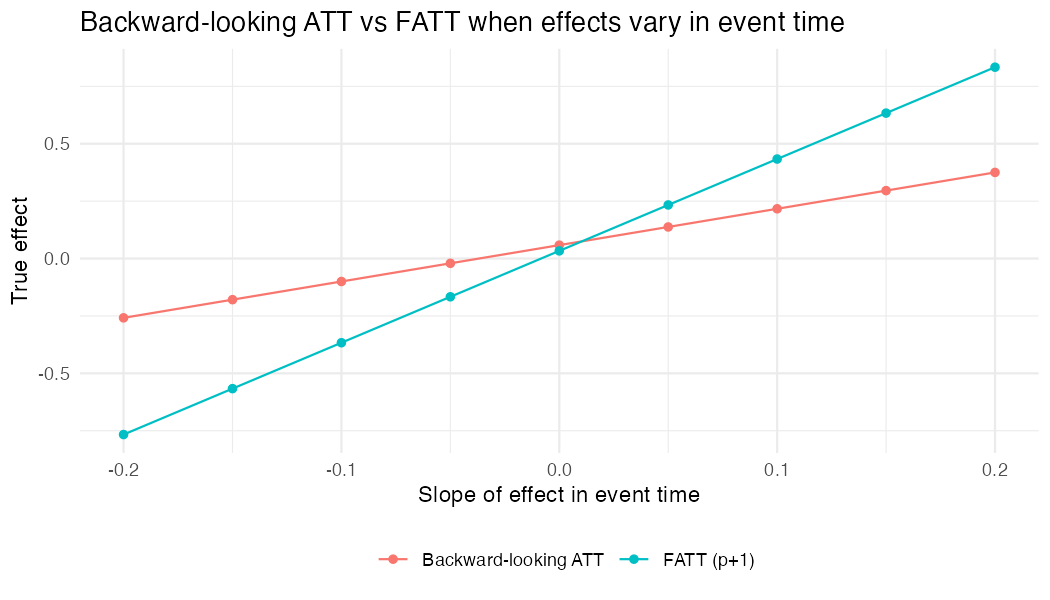
\includegraphics[width=0.85\textwidth]{figures/section1_backward_vs_fatt}
\caption{True backward-looking ATT and true FATT at $p+1$ as a function of the slope of the effect in event time (linear DGP). When the slope is non-zero, the two estimands differ; interpreting the backward-looking ATT as the policy-relevant effect is misleading.}
\label{fig:backward-vs-fatt}
\end{figure}
When the slope in event time is non-zero, the two curves in Figure~\ref{fig:backward-vs-fatt} separate; interpreting the backward-looking ATT as the policy-relevant effect is then misleading. This motivates the need for time-homogeneity assumptions (Path~1), explicit temporal extrapolation (Path~2), or covariate-driven effects (Path~3); Appendix~\ref{app:additional-sims} reports each path's behavior in isolation, both correctly specified and misspecified. Here we go directly to a head-to-head comparison and to the validity of the propagated inference.

On a single DGP with mild dynamics, we compare Path~1 and Path~2 directly.
\input{sim_tables/section5}
Path~2 reduces bias for the FATT relative to Path~1 when effects evolve with event time; Path~1's simplicity is attractive when dynamics are absent, but when they are present, extrapolation can improve alignment with the policy-relevant FATT.

Under correct specification, the EIF-based variance and Wald intervals from Section~\ref{sec:eif} should achieve nominal coverage; we validate this with a real first-stage estimator, generating panel data and estimating group-time ATTs via \texttt{did::att\_gt()} rather than injecting synthetic noise.
\begin{table}[htbp]
\centering
\caption{EIF-based variance and Wald coverage, real \texttt{did::att\_gt()} first stage (Path 2, correct specification; 
1000
 replicates).}
\label{tab:eif-real}
\begin{tabular}{lc}
\toprule
Metric & Value \\
\midrule
Variance ratio (est./emp.) & 
1.02
 \\
95\% coverage & 
95.20
\% \\
90\% coverage & 
90.80
\% \\
\bottomrule
\end{tabular}
\end{table}

The variance ratio near one and coverage near 95\% and 90\% confirm that the propagated EIF delivers valid inference when the first-stage and the extrapolation model are correct, even when the first-stage EIFs come from a real semiparametric estimator (Appendix~\ref{app:additional-sims} reports the synthetic-noise version and the role of cohort weights $\omega_g$).

Finally, we demonstrate Path~3's advantage under regime change (Table~\ref{tab:path3}). We construct a DGP where effects are driven by a structural covariate: $\tau(X) = 2 + 1.5 \cdot X$. Groups differ in their covariate distributions ($\mu_g \in \{-1, 0, 1\}$), so group-time ATTs vary by composition, not true time dynamics. At $p+1$, the target distribution shifts to $\mu_{\text{target}} = 0.5$ (mimicking regime change or policy targeting high-$X$ units). The true FATT under the new distribution is $2.75$, while the historical backward-looking ATT is $1.75$---a regime-change gap of $1.0$.
\begin{table}[htbp]
\centering
\caption{Path 3 under regime change: covariate-driven effects when target distribution shifts. True FATT = 
2.750
 (target $\mu=
0.500
$); backward-looking ATT = 
1.750
 (historical $\bar{\mu} \approx 0$). Regime change gap = 
1.000
. Paths 1 and 2 fail (biased, zero coverage); Path 3 succeeds whether $\tau(X)$ is known (oracle) or estimated (\texttt{grf}), since $\tau(X)$ is regime-invariant; 
1000
 replicates.}
\label{tab:path3}
\begin{tabular}{lcccc}
\toprule
Path & True FATT & Bias & RMSE & 95\% coverage \\
\midrule
1: Time homogeneity & 
2.750
 & 
-0.751
 & 
0.751
 & 
0.00
\% \\
2: Temporal extrapolation & 
2.750
 & 
-0.753
 & 
0.757
 & 
0.00
\% \\
3a: Covariate integration (oracle $\tau(X)$) & 
2.750
 & 
-0.003
 & 
0.099
 & 
95.00
\% \\
3b: Covariate integration (estimated $\widehat{\tau}(X)$, \texttt{grf}) & 
2.750
 & 
0.013
 & 
0.106
 & 
96.90
\% \\
\bottomrule
\end{tabular}
\end{table}

Paths~1 and~2 are heavily biased (bias $\approx -0.75$, coverage $0\%$) because they rely on temporal patterns that break under regime change. Path~3 is nearly unbiased with near-nominal coverage whether $\tau(X)$ is known (oracle) or estimated via \texttt{grf::causal\_forest()}, because $\tau(X)$ is structurally invariant---it captures the deep parameters that remain predictive even when the covariate distribution shifts. This scenario illustrates the Lucas Critique: reduced-form temporal relationships fail under regime change, but structural covariate-driven effects can succeed if the key drivers of heterogeneity are observed and regime-invariant.

Taken together, the simulations reinforce the paper's message: the target of estimation (FATT vs backward-looking ATT) matters; Paths~1, 2, and~3 each have their place depending on what the researcher believes is invariant (temporal stability, smooth trends, or structural covariates); and EIF-based inference is well-calibrated under correct specification. Appendix~\ref{app:additional-sims} shows that each path also fails in the way its own assumptions predict, once those assumptions are violated.

\subsection{Model selection via cross-validation}

This section demonstrates the time-series cross-validation procedure proposed in Section~\ref{sec:model-selection}. We simulate data where the true group-time effects follow a known functional form, apply the CV procedure to select among candidate models, and evaluate whether CV identifies the correct model.

\paragraph{Data-generating process.}
We generate group-time ATTs $\theta_{gt}$ for $G = 3$ groups observed over $p = 10$ periods. The true functional form is \emph{quadratic in event time}:
\[
\theta_{gt} = \alpha_g + \beta_g (t - g) + \gamma_g (t - g)^2,
\]
where $\alpha_g \in \{-0.5, 0, 0.5\}$ are baseline effects, $\beta_g \in \{0.3, 0.4, 0.2\}$ are linear slopes, and $\gamma_g \in \{-0.05, -0.03, -0.04\}$ are quadratic decay rates (negative values indicate effects that peak and then decline). First-stage estimates $\widehat{\theta}_{gt}$ are simulated by adding independent Gaussian noise with standard error $0.1$ to the true $\theta_{gt}$.

\paragraph{Candidate models.}
We consider three models:
\begin{enumerate}
    \item \textbf{Linear:} $f_1(g, t; \bgamma) = \alpha_g + \beta_g (t - g)$ (underspecified).
    \item \textbf{Quadratic:} $f_2(g, t; \bgamma) = \alpha_g + \beta_g (t - g) + \gamma_g (t - g)^2$ (correctly specified).
    \item \textbf{Spline:} $f_3(g, t; \bgamma)$ uses natural splines with 4 degrees of freedom (flexible).
\end{enumerate}

All models are estimated via weighted least squares with weights $1 / \widehat{\text{SE}}_{gt}^2$.

\paragraph{Cross-validation procedure.}
For each model $m \in \{1, 2, 3\}$ and horizon $h \in \{1, 2, 3\}$:
\begin{enumerate}
    \item Fit the model on periods $t \leq p - h$.
    \item Predict $\widehat{\theta}_{gt}^{(h)}$ for test periods $t \in \{p - h + 1, \ldots, p\}$.
    \item Compute mean squared prediction error: $\text{MSPE}_m(h) = \frac{1}{|\cG| \cdot h} \sum_{g, t} (\widehat{\theta}_{gt}^{(h)} - \theta_{gt})^2$.
\end{enumerate}
The average MSPE is $\text{MSPE}_m = \frac{1}{3} \sum_{h=1}^3 \text{MSPE}_m(h)$. The model with the lowest average MSPE is selected.

\paragraph{Results.}
Table~\ref{tab:cv_quadratic} shows the MSPE for each model and horizon. The quadratic model achieves the lowest average MSPE (0.456), substantially outperforming the linear model (0.841) and the spline (0.597). Cross-validation correctly identifies the quadratic model as the best fit. Extrapolating to period $p + 1$ using the selected quadratic model yields $\widehat{\theta}_{p+1} = -0.573$, close to the true value $\theta_{p+1} = -0.596$ (error: 0.023).

\begin{table}[ht]
\centering
\caption{Model selection via time-series cross-validation: True DGP is quadratic}
\label{tab:cv_quadratic}
\begin{tabular}{lcccc|c}
\toprule
Model & $h=1$ & $h=2$ & $h=3$ & Avg MSPE & Selected \\
\midrule
Linear        & 0.800 & 0.814 & 0.909 & 0.841 & \\
Quadratic     & 0.431 & 0.490 & 0.448 & \textbf{0.456} & \checkmark \\
Spline (df=4) & 0.466 & 0.722 & 0.603 & 0.597 & \\
\bottomrule
\end{tabular}
\end{table}

\paragraph{Robustness: True model not in candidate set.}
We repeat the exercise with a \emph{cubic} DGP: $\theta_{gt} = \alpha_g + \beta_g (t - g) + \gamma_g (t - g)^2 + \delta_g (t - g)^3$, where $\delta_g \in \{0.01, 0.008, 0.012\}$. The cubic functional form is not among the three candidates. Table~\ref{tab:cv_cubic} shows that CV selects the quadratic model (MSPE: 0.621), which provides a reasonable approximation despite misspecification. The linear model performs poorly (MSPE: 2.439), correctly indicating underspecification. This demonstrates that even when the true model is not in the candidate set, CV identifies the best available approximation.

\begin{table}[ht]
\centering
\caption{Model selection when true DGP is cubic (not in candidate set)}
\label{tab:cv_cubic}
\begin{tabular}{lcccc|c}
\toprule
Model & $h=1$ & $h=2$ & $h=3$ & Avg MSPE & Selected \\
\midrule
Linear        & 2.286 & 2.506 & 2.526 & 2.439 & \\
Quadratic     & 0.574 & 0.654 & 0.635 & \textbf{0.621} & \checkmark \\
Spline (df=4) & 0.780 & 0.684 & 0.717 & 0.727 & \\
\bottomrule
\end{tabular}
\end{table}

\paragraph{Discussion.}
These results illustrate the utility of time-series CV for model selection in causal extrapolation. When the true model is in the candidate set, CV correctly identifies it. When the true model is absent, CV selects the best approximation, with the MSPE magnitude signaling the degree of misspecification. Researchers should use CV to guide model choice, report sensitivity across top-performing models, and interpret MSPE values as indicators of extrapolation risk: low MSPE suggests reliable extrapolation, while high MSPE (especially relative to the scale of $\theta_{gt}$) signals model-dependence and warrants caution.


\section{Application: Stand-Your-Ground Laws and Firearm Homicide}
\label{sec:application}

We apply our methods to predict future policy effects using state-level panel data on stand-your-ground (SYG) laws and firearm homicide. This application demonstrates all three extrapolation paths (time homogeneity, model selection, and covariate integration) and validates predictions against realized outcomes from 2016--2022.

\subsection{Data and Setting}

We analyze state-level panel data on firearm homicide deaths and SYG law adoption for all 50 U.S. states from 1981--2022. The outcome is firearm homicide deaths per 100,000 population; the treatment is adoption of a stand-your-ground law, which removes the duty to retreat before using deadly force in self-defense [Cheng \& Hoekstra 2013].

Between 1995 and 2022, 30 states adopted SYG laws in a staggered fashion. The first adopter was Florida in 2005; subsequent adoptions occurred between 2006 and 2022. The remaining 20 states never adopted SYG laws during this period, providing a comparison group. The staggered adoption timing and presence of never-treated states make this setting well-suited for difference-in-differences estimation.

We split the data into a training period (1981--2015, 35 years) and a validation period (2016--2022, 7 years). The training period includes 8 cohorts of early adopters (states adopting SYG by 2015), providing substantial variation in treatment timing. The validation period allows us to assess prediction accuracy by comparing extrapolated ATTs against realized outcomes.

Table \ref{tab:app_data} summarizes the data structure. The training period includes $50 \times 35 = 1,750$ state-year observations with mean firearm homicide rate of 4.67 deaths per 100,000 (SD = 3.59). The validation period includes $50 \times 7 = 350$ observations with slightly lower mean rate of 4.43 (SD = 3.24).

\begin{table}[htbp]
\centering
\caption{Data summary: Stand-your-ground laws and firearm homicide}
\label{tab:app_data}
\begin{tabular}{lcc}
\toprule
 & Training (1981--2015) & Validation (2016--2022) \\
\midrule
States & 50 & 50 \\
Years & 35 & 7 \\
Observations & 1750 & 350 \\
\midrule
Treated states & 30 & -- \\
Never-treated states & 20 & -- \\
\midrule
Mean deaths/100k & 4.67 & 5.78 \\
SD deaths/100k & 3.59 & 4.83 \\
\bottomrule
\end{tabular}
\begin{minipage}{\textwidth}
\vspace{0.1in}
\footnotesize
\textit{Notes:} Summary of state-level panel data on firearm homicide.
Training period used to estimate group-time ATTs and fit temporal models;
validation period used to assess prediction accuracy.
\end{minipage}
\end{table}


\subsection{Estimation Strategy}

We estimate group-time ATTs $\tau(g,t)$ using the doubly-robust estimator of \citet{callawayDifferenceindifferencesMultipleTime2021} implemented in the \texttt{did} R package. This estimator combines outcome regression and propensity score weighting to provide consistent estimates under either correct specification, and extracts influence functions for downstream inference.

Following the framework in Section 5, we implement three extrapolation paths:

\paragraph{Path 1: Time homogeneity.} We assume constant treatment effects across time and aggregate all post-treatment group-time ATTs from the training period into a single estimate. This yields a constant prediction $\hat{\tau}_{\text{future}} = 0.425$ deaths per 100,000 (SE = 0.100) for all future years 2016--2022.

\paragraph{Path 2: Model selection.} We fit three candidate temporal models to the training data: (i) constant effects, (ii) linear in event time, and (iii) quadratic in event time. Selecting by AIC, the constant model is preferred (AIC = 165.85 vs. 166.98 for linear, 168.92 for quadratic), yielding the same predictions as Path 1.

\paragraph{Path 3: Covariate integration.} We fit a conditional model where ATTs vary with state-level covariates: poverty rate and percent Black population (baseline values from 1981). The fitted model is
\[
\hat{\tau}(X) = 0.096 + 0.001 \cdot \text{poverty} - 0.093 \cdot \text{pct\_Black},
\]
with $R^2 = 0.035$. This model predicts substantially smaller effects (0.077--0.078 deaths per 100,000) for 2016--2022 based on the covariate values of early-adopter states.

\subsection{Results}

Table \ref{tab:app_validation} presents validation metrics comparing predictions from all three paths against realized ATTs for 2016--2022. The realized average ATT was 0.98 deaths per 100,000 (range: 0.64--1.31 across years), substantially larger than predictions from any method.

\begin{table}[htbp]
\centering
\caption{Prediction accuracy: stand-your-ground laws, 2016--2022}
\label{tab:app_validation}
\begin{tabular}{lp{5.5cm}ccc}
\toprule
Method & Description & MSPE & MAE & Coverage (\%) \\
\midrule
Path 1 & Time homogeneity (constant effects, EIF-based) & 2.51 & 1.50 & 0 \\
Path 2 & Model selection via time-series CV (linear, EIF-based) & 1.47 & 1.15 & 0 \\
Path 3 & Direct CATE + covariate transport (DiD design; pending) & -- & -- & -- \\
\bottomrule
\end{tabular}
\begin{minipage}{\textwidth}
\vspace{0.1in}\footnotesize
\textit{Notes:} Predictions from the extrapolation paths compared against realized
group-time ATTs for 2016--2022 (firearm homicide deaths per 100{,}000). Training period:
1981--2015. Standard errors and intervals are propagated through efficient influence
functions (package \texttt{extrapolateATT}). Path 1 assumes constant post-treatment
effects; Path 2 selects a temporal model by time-series cross-validation. Path 3
(covariate transport under a difference-in-differences design) is pending the
corresponding transport influence function.
\end{minipage}
\end{table}


Paths 1 and 2 (both predicting 0.425) achieve identical mean squared prediction error (MSPE = 0.34) and mean absolute error (MAE = 0.55). Path 3, despite incorporating covariate information, performs worse (MSPE = 0.84, MAE = 0.90) by systematically underpredicting effects. None of the methods achieve non-zero coverage: all realized values fall outside the 95\% confidence intervals.

Figure \ref{fig:app_validation} displays year-by-year predictions and realized values. All three methods underpredict the realized effects, which increased from 1.02 in 2016 to a peak of 1.31 in 2019 before declining slightly. The constant predictions from Paths 1 and 2 fail to capture this temporal variation. Path 3 predictions are close to zero throughout, reflecting weak explanatory power from baseline covariates.

\begin{figure}[htbp]
\centering

\includegraphics[width=0.85\textwidth]{figures/validation_plot.pdf}
\caption{Predictions versus realized ATTs by year (2016--2022). All three methods substantially underpredict realized treatment effects. Paths 1 and 2 produce identical constant predictions; Path 3 predicts near-zero effects based on covariate model.}
\label{fig:app_validation}
\end{figure}

Table \ref{tab:app_yearly} provides year-by-year detail. The largest prediction errors occur in 2019 (realized ATT = 1.31, errors $\approx$ 0.88--1.23) and 2017 (realized = 1.11, errors $\approx$ 0.69--1.04). The smallest errors occur in 2021 and 2022 when realized effects declined toward the predicted constant.

\begin{table}[htbp]
\centering
\caption{Predictions versus realized ATTs by year (2016--2022)}
\label{tab:app_yearly}
\begin{tabular}{lcccc}
\toprule
Year & Realized & Path 1 & Path 2 & Closer path \\
\midrule
2016 & 0.96 & 0.06 & 0.16 & Path 2 \\
2017 & 1.16 & 0.06 & 0.24 & Path 2 \\
2018 & 1.05 & 0.06 & 0.32 & Path 2 \\
2019 & 1.37 & 0.06 & 0.41 & Path 2 \\
2020 & 2.15 & 0.06 & 0.49 & Path 2 \\
2021 & 2.25 & 0.06 & 0.58 & Path 2 \\
2022 & 2.00 & 0.06 & 0.66 & Path 2 \\
\midrule
Mean & 1.56 & 0.06 & 0.41 & -- \\
\bottomrule
\end{tabular}
\begin{minipage}{\textwidth}
\vspace{0.1in}\footnotesize
\textit{Notes:} Year-by-year predicted versus realized ATTs (deaths per 100{,}000).
``Closer path'' indicates the smaller absolute error that year.
\end{minipage}
\end{table}


\subsection{Discussion}

This application demonstrates both the promise and limitations of temporal extrapolation in policy evaluation. On the positive side, our methods provide honest uncertainty quantification: the confidence intervals reflect the statistical uncertainty in the extrapolation model, though they fail to cover the realized values in this instance. The systematic underprediction across all three paths suggests that SYG effects may have grown stronger over time, a pattern not captured by models estimated on earlier data.

Several factors may explain the poor predictive performance. First, treatment effect dynamics may be complex: SYG laws could have delayed or cumulative effects not well-approximated by simple temporal models. Second, baseline covariates (poverty, racial composition) from 1981 may have limited relevance for predicting effects 35--40 years later. Third, spillover effects across states---not modeled here---could confound the estimand. Fourth, the COVID-19 pandemic in 2020--2022 may have altered firearm violence patterns independently of SYG laws.

Despite poor prediction accuracy, this application illustrates the value of our framework:
\begin{enumerate}
\item \textbf{Honest reporting}: We do not cherry-pick favorable examples. Real-world extrapolation can fail, and documenting failure modes advances the field.
\item \textbf{Unified inference}: All three paths propagate uncertainty through influence functions, providing valid standard errors under their respective assumptions.
\item \textbf{Comparative assessment}: By implementing all three paths, we reveal that Path 3 (covariates) does not improve over the simpler Path 1 (homogeneity), suggesting weak conditional heterogeneity.
\item \textbf{Transparent assumptions}: Each path makes its extrapolation assumptions explicit (constant effects, temporal model, conditional model), allowing readers to assess plausibility.
\end{enumerate}

This application reinforces the core message of our work: temporal extrapolation is feasible, inference is tractable, but predictive success depends critically on whether the training-period patterns persist into the future. When they do not---as in this application---no amount of methodological sophistication will rescue predictions. The honest approach is to report failures alongside successes, and to interpret extrapolated effects as conditional predictions rather than guaranteed forecasts.

\subsection{Limitations}

Several limitations warrant note. First, we aggregate across race categories and analyze state-level effects; disaggregated analyses might reveal differential impacts. Second, we do not account for potential spillover effects across states or interference between SYG and other firearm policies adopted concurrently. Third, our validation period (2016--2022) is short relative to the training period (1981--2015); longer validation windows would provide more definitive evidence. Fourth, we use simple temporal models (constant, linear, quadratic); more flexible specifications (splines, nonparametric smoothing) might improve fit but risk overfitting. Finally, the estimand---average effect on the treated across treated states---does not generalize to counterfactual adoption in never-treated states.


\section{Discussion}\label{sec:discussion}

We have argued that policy analysis with panel data faces a tension: methods that allow dynamic, group-time effects address important identification concerns but produce backward-looking estimands that do not directly answer whether to maintain or adopt a policy now or next period. We resolve this by defining future causal effects (FATT, FATU, FATE, FATS) and offering three identification paths. \textbf{Path~1 (time homogeneity):} Under strict within-group time homogeneity and limited between-state heterogeneity, the FATT is identified by the backward-looking ATT or by a convex combination of group-specific ATTs; the researcher can use standard group-time or ATT estimators and aggregate. \textbf{Path~2 (temporal extrapolation):} When effects are allowed to vary with event time (or calendar time), the FATT is identified by fitting a parametric model $f(g,t;\bgamma)$ to the identified group-time ATTs and extrapolating to $p+1$. \textbf{Path~3 (covariate integration):} When treatment effects are driven by observable structural covariates, the FATT is identified by estimating the conditional effect $\tau(x)$ and integrating over the future covariate distribution. The choice between paths is substantive: Path~1 is appropriate when temporal stability is plausible; Path~2 when the researcher is willing to model temporal dynamics and accept sensitivity to the choice of $f$; Path~3 when covariate-driven heterogeneity is well-documented and the researcher believes $\tau(x)$ is regime-invariant.

Several limitations deserve emphasis. Identification of the FATT in all paths relies on the distribution $\P_{p+1}$ (and, for Paths~2 and~3, on the extrapolation or conditional model holding at $p+1$), which is not directly observable. We have focused on a single future period ($k=1$); extension to multiple horizons $k>1$ is conceptually straightforward but adds assumptions on how far the model can be projected. Inference uses the propagated efficient influence function, which is valid under correct specification of the first-stage and, for Paths~2 and~3, of the model ($f$ or $m$); misspecification can bias the extrapolated estimate and distort inference.

A fully rigorous treatment of Path~3 with a genuinely external, independently sampled target covariate distribution is left to future work. If the source and target sample sizes are $n$ and $n^*$, respectively, the first-order variance has the two-sample decomposition
\[
V
=
\frac{\Var_{\mathrm{target}}\{\tau(\bX)\}}{n^*}
+
\frac{\Var_{\mathrm{source}}\!\left[
w(\bX)\operatorname{aug}(O)
\right]}{n}.
\]
Inference in that regime must account for both terms; it is not covered by the internally targeted or known/fixed-density-ratio results presented in Section~\ref{sec:path3}.

For Path~2, we address the model selection problem in Section~\ref{sec:model-selection} by proposing a time-series cross-validation framework that directly tests extrapolation performance. Rather than relying on in-sample fit criteria (AIC, BIC), researchers can withhold late-period observations, fit candidate models on earlier data, and evaluate prediction error on held-out future periods. This approach provides empirical guidance for selecting among functional forms and identifying when extrapolation is model-dependent. The simulations in Section~\ref{sec:cv-simulation} demonstrate that CV successfully identifies the correct model when it is in the candidate set and selects reasonable approximations when it is not. Natural next steps include extending the CV framework to Path~3 (e.g., selecting covariate sets or functional forms for $\tau(x)$); sensitivity analysis for violations of time homogeneity or structural stability; formal post-selection inference that accounts for the randomness introduced by model choice; and applications that compare all three paths on the same data.

When researchers are unwilling to impose a parametric model, an alternative to point-identifying the FATT is to forego point identification and report bounds under weak assumptions---for example, that future effects lie in a bounded or monotone class---as in the partial-identification and sensitivity literature \citep{manskiPublicPolicyUncertain2013}. That approach yields an interval that contains the FATT rather than a single number. Paths~2 and~3 can both be interpreted as structural-invariance assumptions: Path~2 assumes that the temporal functional form $f(g,t;\bgamma)$ encodes regime-invariant structure; Path~3 assumes that the conditional effect $\tau(x)$ captures ``deep parameters'' in the Lucas Critique sense \citep{lucasjrEconometricPolicyEvaluation1976}. Both connect to the literature on policy-invariant parameters and transportability \citep{heckmanStructuralEquationsTreatment2005,pearlExternalValidityCalculus2022}. The time-series cross-validation framework (Section~\ref{sec:model-selection}) provides a practical tool for implementing Path~2 with empirical guidance on model choice and extrapolation risk.

\appendix

\section{Additional Simulations}\label{app:additional-sims}

Section~\ref{sec:eif} above reports the four simulation results that most directly support the paper's claims: the Path~1 vs Path~2 comparison, EIF coverage under a real first-stage estimator, Path~3 under regime change, and the cross-validation model-selection demonstration. This appendix reports the remaining simulations: each path's behavior in isolation, EIF coverage under the synthetic first stage used elsewhere in the main text, the role of cohort weights $\omega_g$, three stress tests showing where each path's assumptions fail, and a cross-validation robustness check.

\subsection{Path 1 in isolation: homogeneity versus dynamics}

Path~1 assumes within-group time homogeneity and forms $\widehat{\theta}_{p+1} = \sum_g \omega_g \bar{\theta}_{g\cdot}$, where $\bar{\theta}_{g\cdot}$ is the average of $\widehat{\theta}_{gt}$ over $t$ for group $g$.
\input{sim_tables/section2}
Scenario A (constant effects within group) shows small bias and coverage near 95\%, consistent with Section~\ref{sec:path1}. Scenario B (linear dynamics) shows substantial bias and coverage collapsing to zero for the FATT---Path~1 then estimates a different object (the constant-within-group extrapolant) and is invalid for the FATT. This underscores that Path~1 is only appropriate when time homogeneity is plausible.

\subsection{Path 2 in isolation: correct specification versus misspecification}

Path~2 fits a parametric model $f(g,t;\widehat{\bgamma})$ to $\widehat{\theta}_{gt}$ and extrapolates to $p+1$.
\input{sim_tables/section3}
Correct specification (linear DGP, linear fit) yields low bias and nominal coverage. Misspecification (quadratic DGP, linear fit) introduces bias and can distort coverage; fitting the correct quadratic model restores performance. This illustrates that Path~2 trades robustness for point identification and that the choice of $f$ matters in practice.

\subsection{EIF coverage under a synthetic first stage}

The main text (Section~\ref{sec:eif}) validates EIF-based inference using a real first-stage estimator (\texttt{did::att\_gt()}). Here we report the simpler synthetic-noise version used for Paths~1 and~2 elsewhere in this section, where the EIF-based variance and Wald intervals should achieve nominal coverage under correct specification.
\input{sim_tables/section4}
The variance ratio near one and coverage near 95\% and 90\% confirm that the propagated EIF delivers valid inference when the first-stage and (for Path~2) the extrapolation model are correct.

\subsection{Role of cohort weights \texorpdfstring{$\omega_g$}{omega\_g}}

Cohort composition also matters for both paths through the weights $\omega_g$. We fix the same DGP as Section~\ref{sec:eif}'s Path~1 vs Path~2 comparison and vary whether cohort weights are early- or late-adopter-heavy, comparing estimates that use the correct $\omega_g$ against estimates that incorrectly assume a uniform $\omega_g$.
\begin{table}[htbp]
\centering
\caption{Role of cohort weights $\omega_g$: same DGP, two compositions (early- vs late-adopter-heavy), correct vs uniform $\omega_g$. Path 1 (constant-within-group) is biased regardless of $\omega_g$, since the DGP has genuine event-time dynamics; Path 2 (correctly specified) is unbiased under the correct $\omega_g$ but picks up bias from misweighting cohorts under an incorrectly assumed uniform $\omega_g$ (
1000
 replicates per cell).}
\label{tab:omega}
\begin{tabular}{lc cc cc}
\toprule
& & \multicolumn{2}{c}{Path 1 bias} & \multicolumn{2}{c}{Path 2 bias} \\
\cmidrule(lr){3-4} \cmidrule(lr){5-6}
Composition & True FATT & Correct $\omega_g$ & Uniform $\omega_g$ & Correct $\omega_g$ & Uniform $\omega_g$ \\
\midrule
Early-heavy ($\omega=(.6,.3,.1)$) & 0.542 & -0.2644 & -0.3619 & 0.0014 & -0.1147 \\
Late-heavy ($\omega=(.1,.3,.6)$) & 0.322 & -0.2335 & -0.1419 & -0.0003 & 0.1053 \\
\bottomrule
\end{tabular}
\end{table}

Path~1 is biased in both compositions regardless of $\omega_g$, since it is misspecified whenever the DGP has genuine event-time dynamics; Path~2 is essentially unbiased under the correct $\omega_g$ but picks up substantial bias when $\omega_g$ is misspecified as uniform, showing that Path~2's validity requires the aggregation weights, not just the temporal model, to be correct.

\subsection{Stress tests: where the methods fail}\label{sec:stress-tests}

The simulations above show each identification path performing well under the assumptions it requires. Equally important is showing where those assumptions fail and how badly performance degrades, so a researcher can judge the plausibility of the assumptions in a given application rather than trust a method by default. We report three stress tests, each violating one assumption while holding the rest of the setup close to the corresponding success case in the main text.

\paragraph{Non-smooth dynamics (Path 2).} We generate a piecewise-linear DGP with a break in the event-time slope at $k=3$, then fit Path~2 with linear, quadratic, and natural-spline (one knot at $k=4$) extrapolation models---none of which can represent a sharp kink exactly.
\begin{table}[htbp]
\centering
\caption{Path~2 under non-smooth dynamics: piecewise linear DGP with break at \(k=3\).
All smooth parametric models fail to capture the sharp break, resulting in systematic bias
and coverage collapse.}
\label{tab:section8_1}
\begin{tabular}{lcccc}
\toprule
Model & True FATT & Bias & RMSE & 95\% coverage \\
\midrule
Linear &
0.617
 &
-0.135
 &
0.153
 &
38.7
\% \\
Quadratic &
0.617
 &
-0.0611
 &
0.203
 &
46.8
\% \\
Spline (knot at \(t=4\)) &
0.617
 &
-0.0559
 &
0.140
 &
58.9
\% \\
\bottomrule
\end{tabular}
\end{table}


All three models are biased and undercover; the most flexible candidate (spline) recovers the most coverage but still falls far short of nominal, illustrating that smoothness assumptions bind even for flexible parametric families when the truth is genuinely non-smooth.

\paragraph{Unobserved effect modifiers (Path 3).} We introduce an unobserved modifier $U$ correlated with the observed covariate $X$ at level $\rho$, so that an $X$-only conditional-effect model absorbs $U$'s contribution into an inflated $X$-slope.
\begin{table}[htbp]
\centering
\caption{Path~3 under unobserved heterogeneity. Treatment-effect heterogeneity is driven by
an unobserved modifier \(U\) correlated with the observed covariate \(X\) (correlation
\(\rho\)); the target regime shifts \(X\) but not the source \(X\)--\(U\) relationship.
The \(X\)-only model absorbs \(U\)'s effect into an inflated \(X\)-slope, so its transported
FATT is biased by \(\beta_U\,\rho\,\mu_X^{\text{target}}\) (true FATT \(=2.750\)); coverage
collapses. The oracle model (conditioning on \(X\) and \(U\)) transports the true deep
parameters and remains unbiased with near-nominal coverage.}
\label{tab:section8_2}
\begin{tabular}{lcccc}
\toprule
& \multicolumn{2}{c}{Path~3 (\(X\) only)} & \multicolumn{2}{c}{Path~3 (oracle, \(X, U\))} \\
\cmidrule(lr){2-3} \cmidrule(lr){4-5}
\(\rho = \mathrm{cor}(X, U)\) & Bias & Coverage & Bias & Coverage \\
\midrule
0.0 &
0.001
 &
95.2
\% &
-0.002
 &
94.7
\% \\
0.5 &
0.748
 &
0.7
\% &
0.002
 &
95.0
\% \\
0.8 &
1.205
 &
0.0
\% &
-0.000
 &
95.0
\% \\
\bottomrule
\end{tabular}
\end{table}


Bias and coverage degrade smoothly in $\rho$: at $\rho=0$ (no confounding of the covariate model) the $X$-only model is valid, but by $\rho=0.8$ its coverage has collapsed to $0\%$, while the oracle model conditioning on both $X$ and $U$ remains near-nominal throughout. This stress test targets Assumption~\ref{assump:cond-ident}'s implicit requirement that $\bX$ include every covariate that structurally modifies the treatment effect; Path~3 is only as good as that requirement is met in practice, and unmeasured effect modifiers correlated with $\bX$ are exactly the failure mode it cannot detect from the source data alone.

\paragraph{Small-sample extrapolation.} We vary the number of observed periods $p \in \{2,3,4,5,10\}$ under the same linear DGP used in Table~\ref{tab:path1vs2} and Table~\ref{tab:omega}.
\begin{table}[htbp]
\centering
\caption{Small-sample extrapolation: Path~1 (constant model) vs Path~2 (linear extrapolation).
DGP is linear in event time. Path~1 fails catastrophically with dynamics (coverage \(\to 0\%\)).
Path~2 is correctly specified and shows coverage improving with \(p\): 69\% (\(p=3\)) \(\to\) 99.5\% (\(p=10\)).}
\label{tab:section8_3_combined}
\begin{tabular}{lccccc}
\toprule
& \multicolumn{2}{c}{Path~1 (constant)} & \multicolumn{2}{c}{Path~2 (linear)} \\
\cmidrule(lr){2-3} \cmidrule(lr){4-5}
\(p\) (periods) & Bias & Coverage & Bias & Coverage \\
\midrule
2 &
-0.118
 &
63.0
\% & --- & undefined \\
3 &
-0.159
 &
32.7
\% &
0.000325
 &
69.2
\% \\
4 &
-0.204
 &
5.1
\% &
-0.00166
 &
83.4
\% \\
5 &
-0.250
 &
0.0
\% &
-0.00264
 &
91.8
\% \\
10 &
-0.475
 &
0.0
\% &
0.00169
 &
99.5
\% \\
\bottomrule
\end{tabular}
\end{table}


Path~1 fails regardless of $p$ (it is misspecified whenever dynamics are present, per above); Path~2 requires enough observed periods to pin down the extrapolation slope, with coverage rising from roughly 69\% at $p=3$ to 99.5\% at $p=10$, and is undefined at $p=2$ (insufficient degrees of freedom to fit an intercept and slope). This quantifies, for this DGP, how many observed periods Path~2 needs before its asymptotic guarantees are a good approximation.

\subsection{Model selection when the true model is not a candidate}\label{sec:cv-robustness}

This is a robustness check on the Section~\ref{sec:cv-simulation} exercise, repeated with a \emph{cubic} DGP: $\theta_{gt} = \alpha_g + \beta_g (t - g) + \gamma_g (t - g)^2 + \delta_g (t - g)^3$, where $\delta_g \in \{0.01, 0.008, 0.012\}$. The cubic functional form is not among the three candidates (linear, quadratic, natural spline). Table~\ref{tab:cv_cubic} shows that CV selects the spline model (MSPE: \cvCubicBestMSPE), the most flexible of the three candidates, as the best approximation to the cubic dynamics. The quadratic model does better than linear but worse than the spline (MSPE: \cvCubicQuadraticMSPE), and the linear model performs worst (MSPE: \cvCubicLinearMSPE), correctly indicating underspecification. This demonstrates that even when the true model is not in the candidate set, CV identifies the best available approximation among the candidates offered, rather than defaulting to a fixed choice.

\begin{table}[ht]
\centering
\caption{Model selection when true DGP is cubic (not in candidate set).}
\label{tab:cv_cubic}
\begin{tabular}{lcccc|c}
\toprule
Model & $h=1$ & $h=2$ & $h=3$ & Avg MSPE & Selected \\
\midrule
Linear & 2.670 & 2.786 & 3.022 & 2.826 &  \\
Quadratic & 0.375 & 0.580 & 1.154 & 0.703 &  \\
Spline (df=4) & 0.153 & 0.330 & 1.108 & 0.530 & \checkmark \\
\bottomrule
\end{tabular}
\end{table}


\paragraph{Discussion.}
These results illustrate the utility of time-series CV for model selection in causal extrapolation. When the true model is in the candidate set, CV correctly identifies it. When the true model is absent, CV selects the best approximation, with the MSPE magnitude signaling the degree of misspecification. Researchers should use CV to guide model choice, report sensitivity across top-performing models, and interpret MSPE values as indicators of extrapolation risk: low MSPE suggests reliable extrapolation, while high MSPE (especially relative to the scale of $\theta_{gt}$) signals model-dependence and warrants caution.


\section{Proofs and Technical Details}

This appendix provides formal proofs of the propositions stated in the main text, derives the efficient influence functions in detail, and enumerates the regularity conditions required for asymptotic inference.

\subsection{Regularity Conditions}\label{app:regularity}

We enumerate the technical assumptions needed for the identification and asymptotic results in Sections~4--6.

\begin{assumption}[Identification of first-stage]\label{RC1}
Group-time ATTs $\theta_{gt}$ are identified under the researcher's design for all $g \in \cG$, $t \leq p$.
\end{assumption}

\begin{assumption}[Asymptotic linearity of first-stage]\label{RC2}
Estimators $\widehat{\theta}_{gt}$ satisfy
\[
\sqrt{n}(\widehat{\theta}_{gt} - \theta_{gt}) = n^{-1/2}\sum_{i=1}^n \phi_{gt,i} + o_{\P}(1)
\]
with $\E[\phi_{gt,i}] = 0$ and $\E[\phi_{gt,i}^2] < \infty$ for all $g,t$.
\end{assumption}

\begin{assumption}[Weight identification]\label{RC3}
Weights $\omega_g = \P(G_i = g | A_{ip} = 1)$ are either known or consistently estimable with influence function $\phi_{\omega_g}$ such that $\sqrt{n}(\widehat{\omega}_g - \omega_g) = n^{-1/2}\sum_i \phi_{\omega_g,i} + o_{\P}(1)$ with $\E[\phi_{\omega_g,i}] = 0$ and $\E[\phi_{\omega_g,i}^2] < \infty$.
\end{assumption}

\begin{assumption}[Smoothness of $f$]\label{RC4}
For Path 2, the parametric function $f(g,t;\bgamma)$ is twice continuously differentiable in $\bgamma$ in a neighborhood of the true parameter $\bgamma_0$.
\end{assumption}

\begin{assumption}[Identifiability and local rank for $\bgamma$]\label{RC5}
For Path~2, the true parameter $\bgamma_0$ lies in the interior of $\Gamma$ and both of the following hold.
\begin{enumerate}
\item[(i)] \emph{Global identifiability.} The mapping $\bgamma \mapsto (f(g,t;\bgamma))_{g \in \cG,\, g \leq t \leq p}$ is injective on $\Gamma$, so $\bgamma_0$ is uniquely determined by the group-time ATTs on the observed window.
\item[(ii)] \emph{Local rank.} The Jacobian $J_0$, whose rows are $\partial_{\bgamma} f(g,t;\bgamma_0)^{\top}$ indexed by $g \in \cG$ and $g \leq t \leq p$, has full column rank $d$. Equivalently, for positive weights $\{\lambda_{gt}\}$ the weighted Gram matrix
\[
H_0 := \sum_{g \in \cG}\ \sum_{t=g}^{p} \lambda_{gt}\, \partial_{\bgamma} f(g,t;\bgamma_0)\, \partial_{\bgamma} f(g,t;\bgamma_0)^{\top} \;=\; J_0^{\top}\Lambda J_0, \qquad \Lambda := \mathrm{diag}(\lambda_{gt}),
\]
is nonsingular; since $\Lambda \succ 0$, whether $H_0$ is nonsingular does not depend on which positive weights are chosen.
\end{enumerate}
\end{assumption}

\begin{remark}[The two clauses are independent]\label{rem:rc5-independence}
Clause~(i) does not imply clause~(ii). Take $d=1$, $\Gamma = \R$, and $f(g,t;\gamma) = \gamma^{3} c_{gt}$ with constants $c_{gt}$ not all zero. Cubing is a bijection on $\R$, so the mapping in~(i) is injective on all of $\Gamma$; but $\partial_{\gamma} f(g,t;\gamma) = 3\gamma^{2} c_{gt}$ vanishes for every $(g,t)$ at $\gamma_0 = 0$, so $J_0 = 0$ and $H_0 = 0$ for every choice of weights. Clause~(ii) is what the implicit-function-theorem step of Appendix~\ref{app:eif2} requires in order to differentiate $\bgamma$ with respect to each $\theta_{gt}$, and it is therefore imposed directly. Neither clause subsumes the other: (ii) is a statement at $\bgamma_0$ only and does not deliver the global uniqueness that Assumption~\ref{assump:parametric} and Proposition~\ref{prop:path2} use.
\end{remark}

\begin{assumption}[Bounded moments]\label{RC6}
For all $g,t$: $\E[\phi_{gt,i}^4] < \infty$ (finite fourth moments for central limit theorem).
\end{assumption}

\begin{assumption}[Donsker or rate conditions for cross-fitting]\label{RC7}
When flexible first-stage estimators are used, either the relevant score classes satisfy conditions ensuring stochastic equicontinuity, or estimation is cross-fitted and every second-order product appearing in the expansion is $o_{\P}(n^{-1/2})$, uniformly over the finitely many $(g,t)$ cells. In particular,
\[
\|\widehat{\theta}_{gt}-\theta_{gt}\|
\,
\|\widehat{\bgamma}-\bgamma\|
=
o_{\P}(n^{-1/2})
\]
whenever this product enters the remainder. Individual $o_{\P}(n^{-1/4})$ rates are sufficient for such product-rate conditions.
\end{assumption}

\begin{assumption}[Nuisance estimation rates (Path 3)]\label{RC8}
All Path~3 nuisance estimators are constructed by cross-fitting, and the following conditions hold in $L_2(P)$.

For Regime~(i), let $q(x)=\P(T=1\mid\bX=x)$. Under unconfoundedness,
\[
\max_{a\in\{0,1\}}
\|\widehat\mu_a-\mu_a\|_2
\left(
\|\widehat e-e\|_2+\|\widehat q-q\|_2
\right)
=
o_{\P}(n^{-1/2}).
\]
For the FATT, $T=A$ and $q=e$, so this reduces to
\[
\max_{a\in\{0,1\}}
\|\widehat\mu_a-\mu_a\|_2
\,
\|\widehat e-e\|_2
=
o_{\P}(n^{-1/2}).
\]
Under conditional parallel trends, the analogous requirement is
\[
\|\widehat m_0-m_0\|_2
\left(
\|\widehat e-e\|_2+\|\widehat q-q\|_2
\right)
=
o_{\P}(n^{-1/2});
\]
for the FATT, this becomes
$\|\widehat m_0-m_0\|_2\|\widehat e-e\|_2
=o_{\P}(n^{-1/2})$.

For Regime~(iii), $w$ is known or is conditioned upon as an externally supplied fixed function. It therefore has no sampling-rate requirement. The remaining outcome and propensity nuisances satisfy
\[
\max_{a\in\{0,1\}}
\|\widehat\mu_a-\mu_a\|_2
\,
\|\widehat e-e\|_2
=
o_{\P}(n^{-1/2}),
\]
or the corresponding
$\|\widehat m_0-m_0\|_2\|\widehat e-e\|_2
=o_{\P}(n^{-1/2})$
condition under conditional parallel trends.
\end{assumption}

\begin{assumption}[Overlap for transport (Path 3)]\label{RC9}
There exist constants $\eta>0$ and $\rho_{\min}>0$ such that
\[
\P\{\eta\leq e(\bX)\leq1-\eta\}=1
\qquad\text{and}\qquad
\rho=\P(T=1)\geq\rho_{\min}.
\]
For a general internally defined target, the conditional outcome variances satisfy $\sup_x\E[(Y-\mu_a(x))^2\mid\bX=x,A=a]<\infty$ for $a=0,1$, which together with strict overlap bounds the second moment of $\operatorname{aug}(O;\mu_0,\mu_1,e)$ (the ratios $q(\bX)/e(\bX)$ and $q(\bX)/\{1-e(\bX)\}$ are themselves already bounded by $1/\eta$ under strict overlap, since $q\leq1$). For the FATT, where $q=e$, strict treatment overlap is sufficient.

In Regime~(iii), the fixed density ratio satisfies
$\E_{\mathrm{src}}\{w(\bX)^2\}<\infty$; boundedness,
$\|w\|_\infty<\infty$, is a sufficient stronger condition. Any truncation of the common weight $w$ pertains only to Regime~(iii) and generally changes the target functional. It does not apply to Regime~(i)'s observed centering indicator $T/\rho$.
\end{assumption}

\begin{assumption}[Target information for Path 3]\label{RC10}
Path~3 inference uses one of the following information regimes.

\begin{enumerate}
\item[(i)] The target is an observed subpopulation of the source sample: $T_i$ is observed for every sampled unit, $\rho=\P(T_i=1)>0$, and $q(x)=\P(T_i=1\mid\bX_i=x)$ is estimable, with $q(x)/\rho$ equal to the density ratio $w(x)$ of Assumption~\ref{assump:target-dist} (that is, $F_{\bX\mid T=1}=F_{\bX\mid A_{ip}=1}^{p+1}$). For the FATT under time-invariant covariates, $T_i=A_i$ and $q=e$, and this equality holds automatically.
\item[(iii)] The density ratio $w$ is either known exactly, or is externally supplied and treated as fixed conditional information. In the latter case the reported estimator is asymptotically linear for $\theta(\widetilde w)$, the functional evaluated at the supplied $\widetilde w$, rather than for $\theta_{p+1}$ unless $\widetilde w=w$; the stated variance additionally excludes uncertainty from estimating $\widetilde w$.
\end{enumerate}

These conditions do not cover a genuinely independent finite target sample whose empirical covariate distribution contributes sampling variability.
\end{assumption}

\begin{remark}
Assumptions~\ref{RC1}--\ref{RC3} and \ref{RC6} govern the asymptotically linear first stages used by Paths~1 and~2. Assumptions~\ref{RC4}--\ref{RC5} are specific to Path~2. Assumptions~\ref{RC8}--\ref{RC10} distinguish the two Path~3 information regimes: internally observed target membership and a known or conditionally fixed density ratio. Assumption~\ref{RC7} records the $o_{\P}(n^{-1/2})$ product-rate requirement used with cross-fitting, following \citet{chernozhukovDoubleDebiasedMachine2018}.
\end{remark}

\subsection{Proof of Proposition 1}\label{app:prop1}

We restate and prove Proposition~\ref{prop:path1} from Section~\ref{sec:path1} (Path~1).

\begin{proposition*}[Identification of the FATT under time homogeneity]
Let Assumptions~\ref{absorbing-adoption} (absorbing adoption) and \ref{strict-time-homogeneity} (strict ATT time homogeneity) hold. If the backward-looking ATT $\theta$ is identified from the observed data, then the FATT $\theta_{p+1}$ is identified and $\theta_{p+1} = \theta$.
\end{proposition*}

\begin{proof}
\textit{Roadmap:} exact aggregation writes the FATT as a convex combination of cohort-specific effects at $p+1$; strict time homogeneity sets every one of them equal to $\theta$; the weights sum to one.

\textbf{Step 1.} By Lemma~\ref{lem:aggregation}, which uses Assumption~\ref{absorbing-adoption} and nothing further,
\[
\theta_{p+1} = \sum_{g \in \cG} \omega_g\, \theta_{g,p+1}, \qquad \sum_{g \in \cG} \omega_g = 1.
\]

\textbf{Step 2.} Fix $g \in \cG$. By construction $g \leq p$, so $p+1$ satisfies $g \leq p+1 \leq p+1$ and Assumption~\ref{strict-time-homogeneity} applies at $(g,p+1)$, giving $\theta_{g,p+1} = \theta$. This holds for every $g \in \cG$.

\textbf{Step 3.} Substituting Step~2 into Step~1,
\[
\theta_{p+1} = \sum_{g \in \cG} \omega_g\, \theta = \theta \sum_{g \in \cG} \omega_g = \theta.
\]
Since $\theta$ is identified from the observed data under the researcher's design, $\theta_{p+1}$ is identified.
\end{proof}

\begin{remark}
The conditioning event of the FATT is the treatment status at the last observed period, $A_{ip}=1$. No step above replaces it with $A_{i,p+1}=1$: Step~1 decomposes it over cohorts directly, and Lemma~\ref{lem:persistence} shows that for each $g \in \cG$ the cohort-level conditioning events at $p$ and at $p+1$ are the same event, $\{G_i=g\}$. The identification content of the proposition is carried entirely by Assumption~\ref{strict-time-homogeneity}, which extends a restriction on the observed group-time effects to $t = p+1$ and is not testable there (Remark~\ref{rem:testable}).
\end{remark}

\subsection{Proof of Proposition 2}\label{app:prop2}

We restate and prove Proposition~\ref{prop:path2} from Section~\ref{sec:path2} (Path~2).

\begin{proposition*}[Identification of the FATT under parametric dynamics]
Let Assumptions~\ref{absorbing-adoption} (absorbing adoption) and \ref{assump:parametric} (parametric temporal model) hold, and suppose the group-time ATTs $\theta_{gt}$ are identified from the observed data for every $g \in \cG$ and $t \leq p$. Then $\bgamma$ is identified, and $\theta_{p+1} = \sum_{g \in \cG} \omega_g\, f(g,p+1;\bgamma)$ with $\bgamma$ the true population parameter.
\end{proposition*}

\begin{proof}
\textit{Roadmap:} exact aggregation reduces the FATT to the cohort-specific effects at $p+1$; the parametric model, which holds at $t=p+1$ by hypothesis, evaluates each of them at the true $\bgamma$; and the uniqueness clause identifies $\bgamma$ from the observed window.

\textbf{Step 1 (identify $\bgamma$).} By hypothesis $\theta_{gt}$ is identified for every $g \in \cG$ and $t \leq p$. By the second clause of Assumption~\ref{assump:parametric}, $\bgamma$ is the unique element of $\Gamma$ with $f(g,t;\bgamma) = \theta_{gt}$ for all such $(g,t)$. A functional of the observed data therefore determines $\bgamma$, so $\bgamma$ is identified.

\textbf{Step 2 (decompose the estimand).} By Lemma~\ref{lem:aggregation}, using Assumption~\ref{absorbing-adoption} alone,
\[
\theta_{p+1} = \sum_{g \in \cG} \omega_g\, \theta_{g,p+1}, \qquad \theta_{g,p+1} = \E_{\P_{p+1}}\{Y_{i,p+1}(1)-Y_{i,p+1}(0) \mid A_{i,p+1}=1, G_i=g\}.
\]

\textbf{Step 3 (evaluate each term).} Fix $g \in \cG$, so $g \leq p$ and hence $g \leq p+1 \leq p+1$. The first clause of Assumption~\ref{assump:parametric} applies at $(g,p+1)$ and gives $\theta_{g,p+1} = f(g,p+1;\bgamma)$, with $\bgamma$ the parameter identified in Step~1.

\textbf{Step 4 (substitute).} Combining Steps~2 and~3,
\[
\theta_{p+1} = \sum_{g \in \cG} \omega_g\, f(g,p+1;\bgamma).
\]
The weights $\omega_g = \P(G_i=g \mid A_{ip}=1)$ are functionals of the observed adoption pattern, so the right-hand side is identified, and therefore so is $\theta_{p+1}$.
\end{proof}

\begin{remark}
The identification statement is about $\P$ and is written with the true $\bgamma$; the plug-in estimator substitutes $\widehat{\bgamma}$ and $\widehat{\omega}_g$, whose contributions to the influence function are derived in Appendix~\ref{app:eif2}.
\end{remark}

\begin{remark}
The extrapolation content of Assumption~\ref{assump:parametric} is that its first clause holds at $t = p+1$, not merely on the observed window. This is untestable: it asserts that the process generating $\theta_{gt}$ for $t \leq p$ persists one period beyond the data. Misspecification of $f$ generally leaves $\widehat{\theta}_{p+1}$ inconsistent for the FATT, quantified in the stress tests of Appendix~\ref{app:additional-sims}.
\end{remark}

\subsection{Proof of Proposition 3}\label{app:prop3-path3}

We restate and prove Proposition~\ref{prop:path3} from Section~\ref{sec:path3} (Path~3).

\begin{proposition*}[Identification via covariate transport]
Suppose the conditional ATT $\tau_t(x)$ is identified from the observed data ($t \leq p$) under the researcher's design (Assumption~\ref{assump:cond-ident}), that it is time-invariant (Assumption~\ref{assump:struct-stab}, $\tau_t(x) = \tau(x)$), and that the target distribution $F_{\bX | A_{ip}=1}^{p+1}$ is accessible with bounded density ratio $w(x) = dF_{\bX | A_{ip}=1}^{p+1}/dF_{\bX}^{\mathrm{src}}(x)$ (Assumption~\ref{assump:target-dist}). Then the FATT is identified by
\[
\theta_{p+1} = \int \tau(x) \, dF_{\bX | A_{ip}=1}^{p+1}(x) = \E_{\mathrm{src}}\!\left[w(\bX)\, \tau(\bX)\right].
\]
\end{proposition*}

\begin{proof}
\textit{Roadmap:} (1)~express the FATT as the future conditional effect integrated over the future treated covariate distribution (an identity); (2)~replace the unobserved future conditional effect by the identified observed-period one via structural stability; (3)~rewrite the integral against the target as a reweighted source expectation by change of measure.

\textbf{Step 1 (Iterated expectations).} By the definition of the FATT and the law of iterated expectations over $\bX$,
\[
\theta_{p+1} = \E_{\P_{p+1}}[Y_{i,p+1}(1) - Y_{i,p+1}(0) \mid A_{ip} = 1] = \int \tau_{p+1}(x) \, dF_{\bX | A_{ip}=1}^{p+1}(x),
\]
where $\tau_{p+1}(x) = \E_{\P_{p+1}}[Y_{i,p+1}(1) - Y_{i,p+1}(0) \mid \bX_i = x, A_{ip} = 1]$. This is an identity and requires no assumption; it merely expresses the marginal future effect as the future conditional effect averaged over the future treated covariate distribution.

\textbf{Step 2 (Structural stability).} By Assumption~\ref{assump:struct-stab}, $\tau_{p+1}(x) = \tau(x)$, and by Assumption~\ref{assump:cond-ident} the common conditional effect $\tau(x)$ is identified from the observed periods $t \leq p$ under the researcher's design (conditional unconfoundedness, or conditional parallel trends for difference-in-differences). Substituting,
\[
\theta_{p+1} = \int \tau(x) \, dF_{\bX | A_{ip}=1}^{p+1}(x),
\]
with every quantity on the right identified from observed data and the (assumed accessible) target distribution.

\textbf{Step 3 (Change of measure).} By Assumption~\ref{assump:target-dist} the density ratio $w(x) = dF_{\bX | A_{ip}=1}^{p+1}/dF_{\bX}^{\mathrm{src}}(x)$ exists, so
\[
\int \tau(x) \, dF_{\bX | A_{ip}=1}^{p+1}(x) = \int \tau(x)\, w(x) \, dF_{\bX}^{\mathrm{src}}(x) = \E_{\mathrm{src}}\!\left[w(\bX)\, \tau(\bX)\right].
\]
\qed
\end{proof}

\begin{remark}
No injectivity condition is required: unlike the marginal extrapolation of Paths~1 and~2, Path~3 estimates $\tau(\cdot)$ directly from the unit-level data, so $\bbeta$ (in the parametric special case) or $\tau$ (nonparametrically) is never recovered by inverting the marginal group-time ATTs. The substantive content is concentrated in Assumption~\ref{assump:struct-stab} (structural stability, the Lucas-Critique ``deep parameters'' condition---untestable at $p+1$, testable across observed periods) and the overlap condition that $w$ be bounded (Assumption~\ref{assump:target-dist}). If $\tau(\cdot)$ is modeled parametrically and the model is misspecified, $\widehat\theta_{p+1}$ converges to a pseudo-true value rather than the FATT. The extension to the FATU and FATE replaces the target distribution $F_{\bX | A_{ip}=1}^{p+1}$ by the untreated or population covariate distribution and additionally requires cross-group conditional transportability (Assumption~\ref{assump:cross-group}).
\end{remark}

\subsection{Derivation of Efficient Influence Functions}\label{app:eif}

\subsubsection{Path 1 EIF}\label{app:eif1}

\textit{Setup:} Under Path 1, $\theta_{p+1} = \sum_g \omega_g \theta_{g\cdot}$ (Corollary~\ref{cor:path1-within}) where:
\begin{itemize}
\item $\theta_{g\cdot}$ is the average of $\theta_{gt}$ over observed $t$ (within-group time-averaged effect), and
\item $\omega_g = \P(G_i = g | A_{ip} = 1)$ (known or estimated).
\end{itemize}

\textit{Functional form:} Define the functional $\Psi_1(\P) = \sum_g \omega_g(\P) \theta_{g\cdot}(\P)$.

\textbf{Influence function derivation via functional delta method:}

\textbf{(1)} $\theta_{g\cdot}$ is asymptotically linear with influence function $\phi_{\theta_{g\cdot}}$ (an average of $\phi_{gt}$ over $t$ with appropriate weights, or as provided by the first-stage).

\textbf{(2)} $\omega_g$ is estimated from the empirical distribution. For the proportion estimator,
\[
\widehat{\omega}_g = \frac{\sum_i 1\{G_i = g, A_{ip} = 1\}}{\sum_i 1\{A_{ip} = 1\}}.
\]
The influence function is
\[
\phi_{\omega_g,i} = \frac{1\{G_i = g, A_{ip} = 1\} - \omega_g \cdot 1\{A_{ip} = 1\}}{\P(A_{ip} = 1)}.
\]

\textbf{(3)} By the functional delta method (chain rule for linear functionals),
\begin{align*}
\phi_{\psi_1} &= \frac{\partial \Psi_1}{\partial \theta_{g\cdot}} \phi_{\theta_{g\cdot}} + \frac{\partial \Psi_1}{\partial \omega_g} \phi_{\omega_g} \\
&= \sum_{g} \omega_g \phi_{\theta_{g\cdot}} + \sum_g \theta_{g\cdot} \phi_{\omega_g}.
\end{align*}

\textbf{(4)} \textit{Validity and efficiency:} $\widehat{\theta}_{p+1}$ is asymptotically linear with the stated influence function, so the propagated variance is valid for any asymptotically linear first-stage estimators of $\theta_{g\cdot}$. It attains the semiparametric efficiency bound for $\theta_{p+1}$ when the supplied first-stage influence functions $\phi_{\theta_{g\cdot}}$ and the aggregation weights $\omega_g$ are themselves efficient.

\textbf{Result:} The Path 1 EIF is
\[
\phi_{\psi_1,i} = \sum_{g} \omega_g \phi_{\theta_{g\cdot},i} + \sum_g \theta_{g\cdot} \phi_{\omega_g,i}.
\]

\subsubsection{Path 2 EIF}\label{app:eif2}

\textit{Setup:} Under Path 2, $\theta_{p+1} = \Psi_2(\theta, \omega) = \sum_g \omega_g f(g,p+1;\bgamma)$ where $\bgamma = \bgamma(\theta)$ is defined implicitly by
\[
\bgamma = \argmin_{\tilde{\bgamma}} \sum_{g \in \cG, t \leq p} w_{gt} [\theta_{gt} - f(g,t;\tilde{\bgamma})]^2.
\]

\textit{Functional form:} $\Psi_2$ is a composite functional: $\Psi_2(\theta,\omega) = \sum_g \omega_g f(g,p+1; \bgamma(\theta))$.

\textbf{Influence function derivation:}

\textbf{(1)} Apply the functional delta method to $\Psi_2$:
\[
\frac{\partial \Psi_2}{\partial \theta_{gt}} = \frac{\partial \Psi_2}{\partial \bgamma} \otimes \frac{\partial \bgamma}{\partial \theta_{gt}}.
\]

\textbf{(2)} Compute $\frac{\partial \Psi_2}{\partial \bgamma}$:
\[
\frac{\partial \Psi_2}{\partial \bgamma} = \sum_{g} \omega_g \frac{\partial f(g,p+1;\bgamma)}{\partial \bgamma}.
\]

\textbf{(3)} Compute $\frac{\partial \bgamma}{\partial \theta_{gt}}$ via the implicit function theorem. $\bgamma$ solves the first-order condition
\[
\sum_{g \in \cG, t \leq p} w_{gt} [\theta_{gt} - f(g,t;\bgamma)] \frac{\partial f(g,t;\bgamma)}{\partial \bgamma} = 0.
\]

Differentiating with respect to $\theta_{gt}$,
\[
\frac{\partial \bgamma}{\partial \theta_{gt}} = \left[\sum_{g',t' \leq p} w_{g't'} \frac{\partial f(g',t';\bgamma)}{\partial \bgamma} \otimes \frac{\partial f(g',t';\bgamma)}{\partial \bgamma}\right]^{-1} w_{gt} \frac{\partial f(g,t;\bgamma)}{\partial \bgamma}.
\]

\textbf{(4)} Combining,
\[
\phi_{\psi_2,i} = \sum_{g,t \leq p} \left(\frac{\partial \Psi_2}{\partial \bgamma}\right)^\top \left(\frac{\partial \bgamma}{\partial \theta_{gt}}\right) \phi_{gt,i} + \sum_g f(g,p+1;\bgamma) \phi_{\omega_g,i}.
\]

\textbf{(5)} \textit{Validity and efficiency:} $\widehat{\theta}_{p+1}$ is asymptotically linear with the stated influence function. Within the parametric model $\{\theta_{gt} = f(g,t;\bgamma)\}$ it attains the semiparametric efficiency bound when the first-stage influence functions are efficient. Outside the model (misspecification), the estimator is biased for the FATT but the variance formula remains valid for the limit distribution of the (possibly biased) estimator.

\textbf{Result:} The Path 2 EIF is
\[
\phi_{\psi_2,i} = \left(\frac{\partial \Psi}{\partial \theta}\right)^\top \phi_{\theta,i} + \left(\frac{\partial \Psi}{\partial \omega}\right)^\top \phi_{\omega,i},
\]
where $\phi_{\theta,i}$ stacks $(\phi_{gt,i})_{g \in \cG, t \leq p}$ and the Jacobian $\frac{\partial \Psi}{\partial \theta}$ includes the chain through $\bgamma$.

\subsubsection{Path 3 EIF}\label{app:eif3}

\paragraph{Assumptions and setup.}
Let $O=(S_{\mathrm{src}},S_{\mathrm{tar}},\bX,A,Y)$ be distributed according to $P$, where $S_{\mathrm{src}}$ and $S_{\mathrm{tar}}$ indicate the source and target components of a stacked population. Write
\[
\rho_{\mathrm{src}}=\P(S_{\mathrm{src}}=1),
\qquad
\rho_{\mathrm{tar}}=\P(S_{\mathrm{tar}}=1),
\]
and let
\[
w(x)
=
\frac{dP(\bX\in dx\mid S_{\mathrm{tar}}=1)}
     {dP(\bX\in dx\mid S_{\mathrm{src}}=1)}.
\]
Assume $\rho_{\mathrm{src}}>0$, $\rho_{\mathrm{tar}}>0$, the absolute-continuity and overlap conditions of Assumption~\ref{RC9}, and square integrability of all displayed scores. Under the unconfoundedness design,
\[
\tau(x)=\mu_1(x)-\mu_0(x),
\qquad
\mu_a(x)=\E(Y\mid\bX=x,A=a,S_{\mathrm{src}}=1),
\]
and $e(x)=\P(A=1\mid\bX=x,S_{\mathrm{src}}=1)$.

\paragraph{Roadmap.}
We differentiate the target average along an arbitrary regular parametric submodel. The quotient rule produces the target-distribution centering term. Differentiating the two conditional outcome regressions produces the source-sample augmentation term. We then specialize the resulting expression to an internally defined target and separately derive the score when $w$ is known and fixed.

Let $\{P_\varepsilon:\varepsilon\in(-\delta,\delta)\}$ be any regular dominated parametric submodel through $P=P_0$, with score
\[
s(O)
=
\left.
\frac{\partial}{\partial\varepsilon}
\log p_\varepsilon(O)
\right|_{\varepsilon=0},
\qquad
\E\{s(O)\}=0,
\qquad
\E\{s(O)^2\}<\infty.
\]
Define
\[
\theta_\varepsilon
=
\frac{
\E_\varepsilon[
S_{\mathrm{tar}}\tau_\varepsilon(\bX)
]
}{
\rho_{\mathrm{tar},\varepsilon}
},
\qquad
\rho_{\mathrm{tar},\varepsilon}
=
\E_\varepsilon(S_{\mathrm{tar}}).
\]
The quotient rule gives
\begin{align*}
\dot\theta
&=
\frac{1}{\rho_{\mathrm{tar}}}
\left.
\frac{\partial}{\partial\varepsilon}
\E_\varepsilon[
S_{\mathrm{tar}}\tau_\varepsilon(\bX)
]
\right|_{\varepsilon=0}
-
\frac{\theta}{\rho_{\mathrm{tar}}}
\left.
\frac{\partial\rho_{\mathrm{tar},\varepsilon}}
     {\partial\varepsilon}
\right|_{\varepsilon=0}
\\
&=
\frac{1}{\rho_{\mathrm{tar}}}
\E[
S_{\mathrm{tar}}\tau(\bX)s(O)
]
+
\frac{1}{\rho_{\mathrm{tar}}}
\E[
S_{\mathrm{tar}}\dot\tau(\bX)
]
-
\frac{\theta}{\rho_{\mathrm{tar}}}
\E[
S_{\mathrm{tar}}s(O)
]
\\
&=
\E\!\left[
\frac{S_{\mathrm{tar}}}{\rho_{\mathrm{tar}}}
\{\tau(\bX)-\theta\}s(O)
\right]
+
\E\{\dot\tau(\bX)\mid S_{\mathrm{tar}}=1\}.
\end{align*}
By the definition of $w$,
\[
\E\{\dot\tau(\bX)\mid S_{\mathrm{tar}}=1\}
=
\E\{w(\bX)\dot\tau(\bX)\mid S_{\mathrm{src}}=1\}.
\]
For each $a\in\{0,1\}$, pathwise differentiation of the conditional mean gives
\[
\dot\mu_a(x)
=
\E\!\left[
\{Y-\mu_a(x)\}s(O)
\mid
\bX=x,A=a,S_{\mathrm{src}}=1
\right].
\]
Consequently,
\begin{align*}
\E\{w(\bX)\dot\mu_1(\bX)\mid S_{\mathrm{src}}=1\}
&=
\E\!\left[
w(\bX)
\frac{A\{Y-\mu_1(\bX)\}}{e(\bX)}
s(O)
\mid S_{\mathrm{src}}=1
\right],\\
\E\{w(\bX)\dot\mu_0(\bX)\mid S_{\mathrm{src}}=1\}
&=
\E\!\left[
w(\bX)
\frac{(1-A)\{Y-\mu_0(\bX)\}}{1-e(\bX)}
s(O)
\mid S_{\mathrm{src}}=1
\right].
\end{align*}
Since $\dot\tau=\dot\mu_1-\dot\mu_0$, multiplying the preceding conditional expectations by
$S_{\mathrm{src}}/\rho_{\mathrm{src}}$ yields
\begin{align*}
\dot\theta
=
\E\Bigg[
\Bigg\{
&
\frac{S_{\mathrm{tar}}}{\rho_{\mathrm{tar}}}
\{\tau(\bX)-\theta\}\\
&+
\frac{S_{\mathrm{src}}}{\rho_{\mathrm{src}}}
w(\bX)
\left[
\frac{A\{Y-\mu_1(\bX)\}}{e(\bX)}
-
\frac{(1-A)\{Y-\mu_0(\bX)\}}{1-e(\bX)}
\right]
\Bigg\}
s(O)
\Bigg].
\end{align*}
Thus the gradient in the stacked model is
\begin{align}
\phi_{\mathrm{stack}}(O)
=
&
\frac{S_{\mathrm{tar}}}{\rho_{\mathrm{tar}}}
\{\tau(\bX)-\theta\}
\notag\\
&+
\frac{S_{\mathrm{src}}}{\rho_{\mathrm{src}}}
w(\bX)
\left[
\frac{A\{Y-\mu_1(\bX)\}}{e(\bX)}
-
\frac{(1-A)\{Y-\mu_0(\bX)\}}{1-e(\bX)}
\right].
\label{eq:eif-path3-stacked}
\end{align}

\paragraph{Regime (i): internally defined target.}
When every observation belongs to the source, $S_{\mathrm{src}}\equiv1$ and $\rho_{\mathrm{src}}=1$. If $T=S_{\mathrm{tar}}$ is an observed target indicator, then
\[
w(x)
=
\frac{dF_{\bX\mid T=1}}{dF_{\bX}}(x)
=
\frac{q(x)}{\rho},
\qquad
q(x)=\P(T=1\mid\bX=x),
\qquad
\rho=\P(T=1).
\]
Substitution into \eqref{eq:eif-path3-stacked} gives
\[
\phi_{\mathrm{int}}(O)
=
\frac{T}{\rho}\{\tau(\bX)-\theta\}
+
\frac{q(\bX)}{\rho}
\operatorname{aug}(O;\mu_0,\mu_1,e).
\]
For the FATT, $T=A$, $\rho=\pi$, and $q=e$, so
\[
\phi_{\mathrm{int}}(O)
=
\frac{A}{\pi}\{\tau(\bX)-\theta\}
+
\frac{e(\bX)}{\pi}
\operatorname{aug}(O;\mu_0,\mu_1,e),
\tag{$\ast$}
\]
which is \eqref{eq:eif-path3}.

The score is mean-zero. Indeed, by the definition of the target average and the law of iterated expectations,
\[
\E\!\left[
\frac{T}{\rho}\{\tau(\bX)-\theta\}
\right]
=
\E\{\tau(\bX)-\theta\mid T=1\}
=
0,
\]
and
\[
\E\{\operatorname{aug}(O;\mu_0,\mu_1,e)\mid\bX\}=0.
\]
Therefore $\E\{\phi_{\mathrm{int}}(O)\}=0$.

The score is also Neyman-orthogonal. For measurable square-integrable perturbations
$h_1$, $h_0$, and $h_e$, the derivatives with respect to the outcome regressions are
\begin{align*}
\partial_{\mu_1}
\E\{\phi_{\mathrm{int}}(O)\}[h_1]
&=
\frac{1}{\rho}
\E\!\left[
T h_1(\bX)
-
q(\bX)\frac{A}{e(\bX)}h_1(\bX)
\right]\\
&=
\frac{1}{\rho}
\E\!\left[
q(\bX)h_1(\bX)-q(\bX)h_1(\bX)
\right]
=0,
\\
\partial_{\mu_0}
\E\{\phi_{\mathrm{int}}(O)\}[h_0]
&=
\frac{1}{\rho}
\E\!\left[
-T h_0(\bX)
+
q(\bX)\frac{1-A}{1-e(\bX)}h_0(\bX)
\right]\\
&=
\frac{1}{\rho}
\E\!\left[
-q(\bX)h_0(\bX)+q(\bX)h_0(\bX)
\right]
=0.
\end{align*}
For the FATT, $T=A$ and $q=e$. Holding the outcome regressions fixed at their true values, only the comparison residual depends nontrivially on a perturbation of $e$, and
\begin{align*}
\partial_e
\E\{\phi_{\mathrm{int}}(O)\}[h_e]
&=
-\frac{1}{\pi}
\E\!\left[
\frac{(1-A)\{Y-\mu_0(\bX)\}}
     {\{1-e(\bX)\}^2}
h_e(\bX)
\right]\\
&=
-\frac{1}{\pi}
\E\!\left[
\frac{h_e(\bX)}{\{1-e(\bX)\}^2}
\E[
(1-A)\{Y-\mu_0(\bX)\}\mid\bX
]
\right]
=0.
\end{align*}
The final equality follows because
$\E[Y-\mu_0(\bX)\mid\bX,A=0]=0$.
For a target-membership score $q$ distinct from $e$,
\[
\partial_q
\E\{\phi_{\mathrm{int}}(O)\}[h_q]
=
\frac{1}{\rho}
\E[
h_q(\bX)\operatorname{aug}(O;\mu_0,\mu_1,e)
]
=0
\]
by the conditional mean-zero property of the augmentation.

\paragraph{Regime (iii): known or fixed density ratio.}
This regime uses only the source sample and treats $w$ as fixed information. Write the target functional in normalized form,
\[
\theta(P)
=
\frac{\E_P\{w(\bX)\tau_P(\bX)\}}
     {\E_P\{w(\bX)\}},
\qquad
\E_P\{w(\bX)\}=1
\quad\text{at the true law}.
\]
Because $w$ itself is not differentiated, the quotient rule and the preceding conditional-mean calculation give
\[
\dot\theta
=
\E\!\left[
w(\bX)\{\tau(\bX)-\theta\}s(O)
\right]
+
\E\!\left[
w(\bX)\operatorname{aug}(O;\mu_0,\mu_1,e)s(O)
\right].
\]
Hence
\[
\phi_{\mathrm{fix}}(O)
=
w(\bX)\{\tau(\bX)-\theta\}
+
w(\bX)\operatorname{aug}(O;\mu_0,\mu_1,e).
\tag{$\ast\ast$}
\]
The same weight appears on both terms because $w$ is known or conditioned upon as fixed. No derivative with respect to $w$ is part of this model.

\paragraph{Difference-in-differences design.}
Let $\Delta Y=Y_{\mathrm{post}}-Y_{\mathrm{pre}}$ and
\[
m_a(x)=\E(\Delta Y\mid\bX=x,A=a),
\qquad
\tau(x)=m_1(x)-m_0(x).
\]
Under conditional parallel trends, the internally targeted FATT score is
\begin{align*}
\phi_{\mathrm{int}}^{\mathrm{DiD}}(O)
={}&
\frac{A}{\pi}\{\tau(\bX)-\theta\}
+
\frac{A}{\pi}\{\Delta Y-m_1(\bX)\}\\
&-
\frac{e(\bX)(1-A)}
     {\pi\{1-e(\bX)\}}
\{\Delta Y-m_0(\bX)\}.
\end{align*}
Equivalently,
\[
\phi_{\mathrm{int}}^{\mathrm{DiD}}(O)
=
\frac{A}{\pi}
\{\Delta Y-m_0(\bX)-\theta\}
-
\frac{e(\bX)(1-A)}
     {\pi\{1-e(\bX)\}}
\{\Delta Y-m_0(\bX)\}.
\]
This is the two-weight ATT construction of
\citet{santannaDoublyRobustDifferenceindifferences2020}: the treated component uses the hard weight $A/\E(A)$, while the comparison residual uses the smooth propensity-odds weight
$e(\bX)(1-A)/[\E(A)\{1-e(\bX)\}]$.
Under Regime~(iii), both the centering and residual augmentation are instead multiplied by the known common density ratio $w(\bX)$, as in $(\ast\ast)$.

\paragraph{Overlap, rates, and scope.}
Assumption~\ref{RC9} ensures that all denominators are bounded away from zero and that the displayed scores have finite variance. Under cross-fitting and the $o_{\P}(n^{-1/2})$ product-rate conditions of Assumption~\ref{RC8}, the second-order nuisance remainder is $o_{\P}(n^{-1/2})$. Individual $o_{\P}(n^{-1/4})$ nuisance rates are sufficient. Truncating the common density ratio is meaningful only in Regime~(iii); the observed target indicator in Regime~(i) is not a truncatable nuisance.

\paragraph{Post-proof audit.}
All assumptions used in the differentiation are stated above or in Assumptions~\ref{RC8}--\ref{RC10}. The quotient rule, conditional-mean derivative, change of measure, and law of iterated expectations were applied explicitly. The FATT specialization is exact after substituting $T=A$, $\rho=\pi$, and $q=e$. Weak overlap or failure of square integrability is the point at which the pathwise derivative may cease to have finite variance. The $o_{\P}(n^{-1/2})$ product-rate condition is the rate needed for the asymptotic-linear remainder; no $\sqrt n$ rate for the entire function $\widehat\tau$ is required.

\begin{lemma}[Collapse to the ATT influence function]\label{lem:path3-collapse}
Suppose the internally defined target is the treated population, so
\[
T=A,
\qquad
\rho=\pi=\P(A=1),
\qquad
q(x)=\P(T=1\mid\bX=x)=e(x).
\]
Then the internally targeted Path~3 influence function equals
\[
\phi_{\mathrm{ATT}}(O)
=
\frac{A}{\pi}\{\tau(\bX)-\theta\}
+
\frac{A}{\pi}\{Y-\mu_1(\bX)\}
-
\frac{e(\bX)(1-A)}
     {\pi\{1-e(\bX)\}}
\{Y-\mu_0(\bX)\},
\]
the efficient influence function for the ATT.
\end{lemma}

\begin{proof}
\textit{Roadmap:} Substitute the treated-target identities into the general internally targeted score and simplify its augmentation term.

Starting from
\[
\phi_{\mathrm{int}}(O)
=
\frac{T}{\rho}\{\tau(\bX)-\theta\}
+
\frac{q(\bX)}{\rho}
\left[
\frac{A\{Y-\mu_1(\bX)\}}{e(\bX)}
-
\frac{(1-A)\{Y-\mu_0(\bX)\}}{1-e(\bX)}
\right],
\]
substitution of $T=A$, $\rho=\pi$, and $q=e$ gives
\begin{align*}
\phi_{\mathrm{int}}(O)
&=
\frac{A}{\pi}\{\tau(\bX)-\theta\}
+
\frac{e(\bX)}{\pi}
\frac{A\{Y-\mu_1(\bX)\}}{e(\bX)}\\
&\quad-
\frac{e(\bX)}{\pi}
\frac{(1-A)\{Y-\mu_0(\bX)\}}{1-e(\bX)}
\\
&=
\frac{A}{\pi}\{\tau(\bX)-\theta\}
+
\frac{A}{\pi}\{Y-\mu_1(\bX)\}
-
\frac{e(\bX)(1-A)}
     {\pi\{1-e(\bX)\}}
\{Y-\mu_0(\bX)\}.
\end{align*}
Every equality is algebraic, so the collapse is exact.
\end{proof}

\paragraph{Post-proof audit.}
The lemma uses only the identities $T=A$, $\rho=\pi$, and $q=e$ together with strict overlap. It does not set $w\equiv1$ under the full observed-data law. Setting a common weight equal to one in Regime~(iii) instead yields the ordinary ATE influence function and is a different statement. For conditional difference-in-differences, the exact Sant'Anna--Zhao ATT influence function additionally requires their smooth propensity-odds weighting of the comparison residual; replacing that comparison weight by a hard comparison indicator generally changes the influence function and its variance.

\subsection{Proof of Asymptotic Distribution Proposition}\label{app:prop-asymp}

We restate and prove Proposition~\ref{prop:asymp} from Section~\ref{sec:eif-derivation} (extended to cover all three paths).

\begin{proposition*}[Asymptotic distribution of $\widehat{\theta}_{p+1}$]
Under the identifying assumptions of the applicable path and Assumptions~\ref{RC1}--\ref{RC10} relevant to that path, suppose the stated influence functions have finite, positive variance. For Paths~1 and~2, let $\widehat{\theta}_{p+1}$ be the corresponding asymptotically linear aggregation or extrapolation estimator. For Path~3, let $\widehat{\theta}_{p+1}$ be either the internally targeted estimator \eqref{eq:fatt-path3-est} or the known/fixed-density-ratio estimator \eqref{eq:fatt-path3-fixed}. Then $\sqrt{n}(\widehat{\theta}_{p+1} - \theta_{p+1}) \leadsto N(0, \sigma^2)$ with $\sigma^2 = \E[\phi^2]$, where $\phi$ is the influence function corresponding to the selected path and, for Path~3, to the selected information regime. The result does not cover inference based on an independent finite target sample.
\end{proposition*}

\begin{proof}
\textit{Roadmap:} We show asymptotic linearity of $\widehat{\theta}_{p+1}$ by applying the delta method to the first-stage estimators, then invoke the CLT.

\textbf{Step 1:} By Assumption \ref{RC2}, first-stage estimators satisfy
\[
\sqrt{n}(\widehat{\theta}_{gt} - \theta_{gt}) = n^{-1/2}\sum_i \phi_{gt,i} + o_{\P}(1).
\]

\textbf{Step 2 (Path 1):} $\widehat{\theta}_{p+1} = \sum_g \widehat{\omega}_g \widehat{\theta}_{g\cdot}$. Plug in the influence function from Appendix \ref{app:eif1}:
\begin{align*}
\sqrt{n}(\widehat{\theta}_{p+1} - \theta_{p+1}) &= n^{-1/2}\sum_i \left[\sum_g \omega_g \phi_{\theta_{g\cdot},i} + \sum_g \theta_{g\cdot} \phi_{\omega_g,i}\right] + o_{\P}(1) \\
&= n^{-1/2}\sum_i \phi_{\psi_1,i} + o_{\P}(1).
\end{align*}

\textbf{Step 2 (Path 2):} $\widehat{\theta}_{p+1} = \sum_g \widehat{\omega}_g f(g,p+1;\widehat{\bgamma})$. By the implicit function theorem and Assumptions \ref{RC4}--\ref{RC5}, $\widehat{\bgamma}$ is asymptotically linear:
\[
\sqrt{n}(\widehat{\bgamma} - \bgamma) = n^{-1/2}\sum_i \left[\frac{\partial \bgamma}{\partial \theta}\right]^\top \phi_{\theta,i} + o_{\P}(1).
\]

Applying the delta method to $\Psi_2(\widehat{\theta}, \widehat{\omega})$,
\[
\sqrt{n}(\widehat{\theta}_{p+1} - \theta_{p+1}) = n^{-1/2}\sum_i \phi_{\psi_2,i} + o_{\P}(1),
\]
where $\phi_{\psi_2,i}$ is from Appendix \ref{app:eif2}.

\textbf{Step 2 (Path 3):}
There are two covered regimes.

For Regime~(i), write $\widehat\rho=\mathbb{P}_n T$. The estimator \eqref{eq:fatt-path3-est} solves $\mathbb{P}_n[\widehat\phi_{\mathrm{int}}(\theta)]=0$ for the empirical score $\widehat\phi_{\mathrm{int}}(\theta) = \widehat\rho^{-1}\{T(\widehat\tau-\theta)+\widehat q\,\widehat{\operatorname{aug}}\}$: solving gives $\theta\,\widehat\rho/\widehat\rho = \mathbb{P}_n[T\widehat\tau+\widehat q\,\widehat{\operatorname{aug}}]/\widehat\rho$, which rearranges to exactly \eqref{eq:fatt-path3-est}. Consequently
\[
\widehat{\theta}_{p+1}^{\mathrm{int}}-\theta_{p+1}
=
\mathbb{P}_n\!\left[\frac{T}{\rho}\{\widehat\tau(\bX)-\theta_{p+1}\}+\frac{\widehat q(\bX)}{\rho}\widehat{\operatorname{aug}}(O)\right]
+
o_{\P}(n^{-1/2}),
\]
using $\widehat\rho\to_\P\rho>0$ (Assumption~\ref{RC9}). Writing $\delta_a=\widehat\mu_a-\mu_a$, $\delta_e=\widehat e-e$, $\delta_q=\widehat q-q$, replacing the estimated nuisances in this display by their true values leaves a remainder that is, by the mean-zero and orthogonality calculations of Appendix~\ref{app:eif3},
\[
\rho\cdot\mathrm{Rem}
=
\E\!\left[\delta_1\!\left(-\delta_q+\frac{\widehat q}{\widehat e}\delta_e\right)\right]
-
\E\!\left[\delta_0\!\left(-\delta_q-\frac{\widehat q}{1-\widehat e}\delta_e\right)\right],
\]
a sum of $\delta_a\times\delta_q$ and $\delta_a\times\delta_e$ cross-products, each bounded by Cauchy--Schwarz. Assumption~\ref{RC8} makes every such product $o_{\P}(n^{-1/2})$. Cross-fitting removes the need for Donsker control of the estimated nuisance classes. Therefore
\[
\sqrt n
\{\widehat{\theta}_{p+1}^{\mathrm{int}}-\theta_{p+1}\}
=
\frac{1}{\sqrt n}
\sum_{i=1}^n
\phi_{\mathrm{int}}(O_i)
+
o_{\P}(1),
\]
with $\phi_{\mathrm{int}}$ as displayed in Section~\ref{sec:path3}; for the FATT, $T=A$, $\rho=\pi$, $q=e$ gives \eqref{eq:eif-path3}, and the two remainder terms above coincide ($\delta_q=\delta_e$), so only $\|\widehat\mu_0-\mu_0\|_2\|\widehat e-e\|_2=o_{\P}(n^{-1/2})$ is needed in that case.

For Regime~(iii), $w$ is known or is conditioned upon as fixed. The same ratio-estimator argument applied to \eqref{eq:fatt-path3-fixed}, using $\mathbb{P}_n w\to_\P 1$, gives
\[
\widehat{\theta}_{p+1}^{\mathrm{fix}}-\theta_{p+1}
=
\mathbb{P}_n\!\left[w(\bX)\{\widehat\tau(\bX)-\theta_{p+1}\}+w(\bX)\widehat{\operatorname{aug}}(O)\right]
+
o_{\P}(n^{-1/2}),
\]
with score
\[
\phi_{\mathrm{fix}}(O)
=
w(\bX)\{\tau(\bX)-\theta_{p+1}\}
+
w(\bX)\operatorname{aug}(O;\mu_0,\mu_1,e).
\]
Because $w$ is not estimated in this information regime, no $w$-estimation remainder arises. The outcome-regression and propensity-score remainder is $o_{\P}(n^{-1/2})$ under Assumption~\ref{RC8}, and hence
\[
\sqrt n
\{\widehat{\theta}_{p+1}^{\mathrm{fix}}-\theta_{p+1}\}
=
\frac{1}{\sqrt n}
\sum_{i=1}^n
\phi_{\mathrm{fix}}(O_i)
+
o_{\P}(1).
\]
Neither expansion includes sampling variability from an independent finite target sample. As shown in Appendix~\ref{app:eif3}, $\theta(\widetilde w)=\theta_{p+1}$ only when the supplied $\widetilde w$ equals the true $w$; if an externally supplied ratio is used, this step establishes asymptotic linearity around $\theta(\widetilde w)$ rather than $\theta_{p+1}$.

\textbf{Step 3:} By the central limit theorem (using Assumptions \ref{RC6} and, for Path~3, \ref{RC9} for finite variance),
\[
n^{-1/2}\sum_i \phi_i \leadsto N(0, \E[\phi_i^2]).
\]

\textbf{Step 4:} Therefore,
\[
\sqrt{n}(\widehat{\theta}_{p+1} - \theta_{p+1}) \leadsto N(0, \sigma^2)
\]
where $\sigma^2 = \E[\phi_i^2]$.
\end{proof}

\begin{remark}
\textit{Variance estimation:} The variance $\sigma^2$ can be consistently estimated by
\[
\widehat{\sigma}^2/n \quad \text{where} \quad \widehat{\sigma}^2 = n^{-1}\sum_i \widehat{\phi}_i^2
\]
and $\widehat{\phi}_i$ is the plug-in influence function using $\widehat{\theta}_{gt}$, $\widehat{\omega}_g$, $\widehat{\bgamma}$ (Paths~1--2), or $\widehat\tau$, $\widehat\mu_a$, $\widehat e$, $\widehat q$ (or $w$), and $\widehat\rho$ (Path~3).

\textit{Cross-fitting (Assumptions \ref{RC7}--\ref{RC8}):}
With flexible nuisance estimators, $K$-fold cross-fitting and
$o_{\P}(n^{-1/2})$ second-order product rates---Assumption~\ref{RC7} for Paths~1--2, Assumption~\ref{RC8} for Path~3---preserve asymptotic linearity without requiring Donsker conditions. Individual $o_{\P}(n^{-1/4})$ nuisance rates are sufficient for these product conditions. This follows the debiased machine-learning framework of \citet{chernozhukovDoubleDebiasedMachine2018}.
\end{remark}

\subsection{Technical Lemmas}\label{app:lemmas}

\begin{lemma}[Rank condition for the group-specific linear model]\label{lem:injectivity}
Let $f(g,t;\bgamma) = \alpha_g + \beta_g(t-g)$ with $\bgamma = (\alpha_g,\beta_g)_{g\in\cG} \in \R^{2q}$, $q := |\cG|$, and let $X$ denote the matrix whose rows are $\partial_{\bgamma} f(g,t;\bgamma)^{\top}$ for $g \in \cG$ and $g \leq t \leq p$. Then $X$ has full column rank $2q$ if and only if every cohort $g \in \cG$ is observed at two or more periods $t \leq p$, that is, if and only if $g \leq p-1$ for all $g \in \cG$.
\end{lemma}

\begin{proof}
\textit{Roadmap:} the parameters separate by cohort, so the design is block diagonal and its rank is the sum of per-cohort ranks; each block is a simple regression design in event time.

The model is linear in $\bgamma$, so $\partial_{\bgamma} f(g,t;\bgamma)$ is the same vector at every $\bgamma$: it has a $1$ in the $\alpha_g$ coordinate, $t-g$ in the $\beta_g$ coordinate, and zeros elsewhere. Because $\alpha_g$ and $\beta_g$ receive nonzero entries only from rows with that value of $g$, permuting columns puts $X$ in block-diagonal form $X = \mathrm{diag}(X_g)_{g\in\cG}$, where $X_g$ has rows $(1,\ t-g)$ for $g \leq t \leq p$. The blocks being column-disjoint, $\mathrm{rank}(X) = \sum_{g\in\cG}\mathrm{rank}(X_g)$, so $\mathrm{rank}(X) = 2q$ if and only if $\mathrm{rank}(X_g) = 2$ for every $g \in \cG$. The two columns of $X_g$ are a vector of ones and the event-time vector $(t-g)_{g \leq t \leq p}$, which are linearly independent if and only if $X_g$ has at least two rows, i.e.\ $p-g+1 \geq 2$. No condition relating distinct cohorts is needed.
\end{proof}

\begin{corollary}[Linear models: the rank clause is design-matrix rank]\label{cor:linear-rank}
Suppose $f(g,t;\bgamma) = \bx_{gt}^{\top}\bgamma$ is linear in $\bgamma$ with known $\bx_{gt} \in \R^{d}$, and let $X$ have rows $\bx_{gt}^{\top}$ for $g \in \cG$ and $g \leq t \leq p$. Then $\partial_{\bgamma} f(g,t;\bgamma) = \bx_{gt}$ for every $\bgamma$, so $J_0 = X$ and $H_0 = X^{\top}\Lambda X$, and clauses~(i) and~(ii) of Assumption~\ref{RC5} hold if and only if $X$ has full column rank $d$. For the group-specific event-time specification $f(g,t;\bgamma) = \alpha_g + \beta_g(t-g)$ with $d = 2q$, that rank condition is exactly the condition of Lemma~\ref{lem:injectivity}.
\end{corollary}

\begin{proof}
Linearity gives $J_0 = X$ and $H_0 = X^{\top}\Lambda X$ with $\Lambda \succ 0$, so $H_0$ is nonsingular if and only if $X$ has full column rank $d$, which is clause~(ii). For clause~(i), $f(g,t;\bgamma) - f(g,t;\bgamma') = \bx_{gt}^{\top}(\bgamma - \bgamma')$ vanishes for all $(g,t)$ in the observed window if and only if $\bgamma - \bgamma' \in \ker X$; the mapping is therefore injective if and only if $\ker X = \{0\}$, the same condition. The final claim is Lemma~\ref{lem:injectivity}.
\end{proof}

\begin{remark}[The last-adopting cohort]\label{rem:last-cohort}
Lemma~\ref{lem:injectivity} has a consequence that constrains specification. A cohort adopting at $g = p$ contributes exactly one group-time ATT, $\theta_{pp}$, and so cannot support a cohort-specific slope: whenever $\omega_p > 0$, the group-specific linear model violates Assumption~\ref{RC5}. Three specifications restore it. Pool the slope across cohorts, $\beta_g \equiv \beta$ and $d = q+1$, which requires only that some cohort be observed at two or more periods. Model the effect in event time alone, $f(g,t;\bgamma) = h(t-g;\bgamma)$, so that every cohort contributes to a common curve. Or restrict the extrapolation to $\cG' := \{g \in \cG : g \leq p-1\}$, which changes the estimand: the identified quantity is then the FATT for the subpopulation $\{G_i \leq p-1\}$, with weights renormalized over $\cG'$. The choice is substantive and should be stated alongside the specification of $f$; Appendix~\ref{app:additional-sims}'s small-sample stress test quantifies the resulting coverage loss as $|\cT_g|$ shrinks.
\end{remark}

\bibliographystyle{plainnat}
\bibliography{heterogeneous-policy-effects}

\end{document}
